\chapter{Data-Driven Nonlinear Regulation}%
\label{CH:DATA-DRIVEN-REGULATION}
In this chapter, we collect the basic notions behind the concept of output regulation and data-driven output regulation for nonlinear systems.
The section unfolds as follows, first we introduce, in the simplest possible terms, the problem of output regulation in the
nonlinear context, with an eye to the taxonomy usually adopted in this field.
Then, the next part is devoted to briefly presenting the state-of-the-art of the most consolidated approaches to
the emergent field of \emph{adaptive} nonlinear output regulation and how these techniques can be extended via learning tools, obtaining
a highly robust and flexible solution, able to adapt to a very large class of systems.
The same concepts, notation, and results can also be found in~\cite*{bin2019class, bin2020model, bin2020approximate, gentilini2022adaptive, gentilini2022data}
thus we refer the reader to these works for the complete analysis of the presented results.

%----------------------------------------------------------------------------------------
\section{The Framework of Output Regulation}%
\label{SEC:FRAMEWORK-OUTPUT-REGULATION}
Consider a continuous-time nonlinear system of the form
\begin{equation}%
    \label{EQ:GENERAL-OR-SYSTEM}
    \begin{split}
        \dot{\xx} & = \xfun \lp \ww, \xx, \uu \rp, \\
        \yy & = \yfun \lp \ww, \xx \rp,
    \end{split}
\end{equation}
with state $\xx \in \R^{\dd{\xx}}$, control input $\uu \in \R^{\dd{\uu}}$, measured output $\yy \in \R^{\dd{\yy}}$, and
with $\ww \in \R^{\dd{\ww}}$ exogenous signal generated by an exosystem of the form
\begin{equation}%
    \label{EQ:GENERAL-EXOSYSTEM}
    \dot{\ww} = \wfun \lp \ww \rp.
\end{equation}
The exogenous signal can be treated, in this context, as references to be tracked or disturbances to be rejected.
For this purpose, associated to~\eqqref{EQ:GENERAL-OR-SYSTEM}, there is a set of $\dd{\ee} > 0$ regulation errors
\begin{equation*}
    \ee = \efun \lp \ww, \xx \rp.
\end{equation*}
In this framework, we define the problem of $\eps$-approximate output regulation as the problem to find
an output feedback regulator of the form
\begin{equation}%
    \label{EQ:GENERAL-OR-REGULATOR}
    \begin{split}
        \dot{\xx}_c & = \rfun \lp \xx_c, \yy \rp, \\
        \uu & = \actfun \lp \xx_c, \yy \rp,
    \end{split}
\end{equation}
possibly $\eps$-dependent, with state $\xx_c \in \R^{\dd{\xx_c}}$, such that:
\begin{itemize}
    \item[\emph{Stability.}] The origin of the interconnection between~\eqqref{EQ:GENERAL-OR-SYSTEM} and~\eqqref{EQ:GENERAL-OR-REGULATOR},
    with $\ww = 0$, is asymptotically stable with a domain of attraction $\xset \times \xset_c \in \R^{\dd{\xx}} \times \R^{\dd{\xx_c}}$
    that is an open neighborhood of the origin.
    \item[\emph{Boundedness.}] There exists $\wset \in \R^{\dd{\ww}}$ such that the closed-loop system is uniformly bounded from
    $\wset \times \xset \times \xset_c$.
    \item[\emph{Regulation.}] Each solution to the closed-loop system originating in $\wset \times \xset \times \xset_c$ satisfies
    \begin{equation*}
        \limsup_{t \rightarrow \infty} \| \ee \lp t \rp \| \le \eps.
    \end{equation*}
\end{itemize}
If $\xset$ coincides with $\R^{\dd{\xx}}$, we say that the problem is solved \emph{globally}, otherwise we say that the problem
is solved \emph{locally}. If given each $\xset \subset \R^{\dd{\xx}}$ it is possible to find a possibly $\xset$-dependent regulator 
that solves the problem in $\xset$, we say that the problem is solved \emph{semi-globally}.
If $\eps = 0$, we refer to the problem as the \emph{asymptotic} output regulation problem, while we talk about
\emph{practical} regulation problem whenever, given any $\eps > 0$, there exists a regulator that solves the $\eps$-approximate
output regulation problem. An anchor point in the solution of the above problem is represented by the
steady-state trajectories $\lp \xx^{*}(t), \uu^{*}(t) \rp$, solution of the so-called \emph{regulator equations}
\begin{equation}%
    \label{EQ:GENERAL-REGULATOR-EQUATIONS}
    \begin{split}
        \dot{\ww} & = \wfun \lp \ww \rp, \\ 
        \dot{\xx}^{*} & = \xfun \lp \ww, \xx^{*}, \uu^{*} \rp, \\
        0 & = \efun \lp \ww, \xx^{*} \rp,
    \end{split}
\end{equation}
with $\xx^{*}$ representing the ideal state trajectory associated with a zero regulation error and $\uu^{*}$
the associated input (often referred to as ``the friend'' of $\xx^{*}$).
Regulator structures proposed in the nonlinear context are typically composed of two units, an internal model unit,
and a stabilising unit, with a neat, albeit limiting in many contexts, ``role'' conferred on the two at the design stage:
the former is designed to generate the steady state input $\uu^{*}$ required to keep the error at zero in steady state,
while the latter is designed to steer the closed-loop trajectories of the system to $\xx^{*}$.
What makes the design problem particularly challenging is, of course, the fact that $\lp \xx^{*}(t), \uu^{*}(t) \rp$
are unknown as the initial conditions of~\eqqref{EQ:GENERAL-REGULATOR-EQUATIONS} are such.
Moreover, the sufficient conditions under which asymptotic regulation is ensured are typically expressed by equations
whose analytic solution becomes a hard task even for ``simple'' problems. Moreover, even if a regulator can be constructed,
asymptotic regulation remains a fragile property that is lost at front of slightest plant's or exosystem's perturbation.
The aforementioned problems motivate the researcher to move toward more robust solutions, introducing the concept of adaptive regulation.
In the following we briefly present the two main adaptive approaches to nonlinear regulation designs that have influenced this thesis most strongly,
then we try to extend them via non-supervised learning techniques, to adapt the proposed structure on an ideally infinite class of systems.
The reported regulators embed two different internal models, being a ``post-processing'' the first one and a ``pre-processing'' the second one,
but both apply to multivariable systems. The proposed construction is not ``friend-centric'' but rather it is based on a
``qualitative'' information on the ideal error-zeroing steady state.

%----------------------------------------------------------------------------------------
\section{Identification-Based Post-Processing Internal Model}
\label{SEC:POST-PROCESSING}
In this section, we focus on a subclass of the general regulation problem presented in~\secref{SEC:FRAMEWORK-OUTPUT-REGULATION}
by considering continuous-time nonlinear systems of the form
\begin{equation}%
   \label{EQ:POSTP-FRAMEWORK}
   \begin{split}
      \dot{\zz} &= \zfun(\xx ,\ww) + \zin(\xx, \ww) \uu, \\
      \dot{\chain} &= F \chain + H \last, \\
      \dot{\last} &= \qfun(\xx ,\ww) + \bfun(\xx ,\ww) \uu, \\
      \ee &= C \chain, \hspace{0.5cm} \yy = \text{col}(\chain, \last),
   \end{split}
\end{equation}
in which $\zz \in \R^{\dd{\zz}}$, $\yy \in \R^{\dd{\yy}}$, $\ee \in \R^{\dd{\ee}}$, $\chain \in \R^{\dd{\ee}}$, and,
$\uu \in \R^{\dd{\uu}}$ with $\dd{\uu} \ge \dd{\ee}$. The entire stack of states is denoted here by $\xx = \text{col}(\zz, \chain, \last)$.
Moreover, $\chain = \text{col}(\chain^1, \dots, \chain^{\dd{\ee}})$, with $\chain^i \in \R^{n_{\chain}^i}$, $i = 1, \dots, \dd{\ee}$,
and $\sum_{k=1}^{\dd{\ee}} n_{\chain}^k = n_{\chain}$. The exogenous signal $\ww \in \R^{\dd{\ww}}$ is generated by an exosystem
of the same form of~\eqqref{EQ:GENERAL-EXOSYSTEM}. The matrices $F \in \R^{n_{\chain} \times n_{\chain}}$,
$H \in \R^{n_{\chain} \times \dd{\ee}}$, and $C \in \R^{\dd{\ee} \times n_{\chain}}$ are defined as a block-diagonal matrices with entries
\begin{equation*}
   \begin{matrix}
      F_i =
      \begin{pmatrix}
         0_{(n_{\chain}^i-1) \times 1} & I_{n_{\chain}^i - 1} \\
         0 & 0_{1 \times (n_{\chain}^i-1)}
      \end{pmatrix}, &
      H_i =
      \begin{pmatrix}
         0_{(n_{\chain}^i-1) \times 1} \\ 1
      \end{pmatrix},
   \end{matrix}
\end{equation*}
\begin{equation*}
   C_i =
   \begin{pmatrix}
      1 & 0_{1 \times (n_{\chain}^i-1)}
   \end{pmatrix}.
\end{equation*}
Equation~\eqref{EQ:POSTP-FRAMEWORK} frames the problem of output regulation on a particular class of systems that embraces
a large number of use-cases addressed in literature. In particular, note that all systems presenting \textit{(a)} a well-defined vector
relative degree and admitting a canonical normal form, or that are \textit{(b)} strongly invertible and feedback linearisable,
with respect to the pair $\lp \uu, \ee \rp$, fit inside the proposed framework.
The regulator presented in this section is based on the following standing assumptions (see~\cite[Assumption~A1,~A2]{bin2019class}).
\begin{assumption}%
   There exist $\beta_0 \in \KL$, $\alpha_0 > 0$ and, for each solution $\ww$ of~\eqref{EQ:GENERAL-EXOSYSTEM},
   there exist $\zz\s : \R_{\ge 0} \mapsto \R^{\dd{\zz}}$ and $\uu\s : \R_{\ge 0} \mapsto \R^{\dd{\uu}}$ fulfilling
   \begin{equation}%
      \label{EQ:POSTP-REGULATOR-EQUATIONS}
      \begin{split}
         \dot{\zz}\s & = \zfun(\ww, \xx\s) + \zin(\ww, \xx\s)\uu\s, \\
         0 & = q(\ww, \xx\s) + \bfun(\ww, \xx\s)\uu\s,
      \end{split}
   \end{equation}
   where $\xx\s = \lp\zz\s, 0, 0\rp$, and for all $t > 0$ the following holds
   \begin{equation*}
      \lb \zz(t) - \zz\s(t) \rb \le \beta_0\lp\lb \zz(0) - \zz\s(0) \rb, t\rp + \alpha_0 \lb \lp\chain, \last\rp \rb_{\lps0,t\rp}.
   \end{equation*}
\end{assumption}
\begin{assumption}%
   There exists a full-rank matrix $\LL \in \R^{\dd{\uu} \times \dd{\ee}}$ such that the matrix $\bfun(\ww, \xx)\LL$ is bounded, and
   \begin{equation*}
      \LL\T \bfun(\ww, \xx)\T + \bfun(\ww, \xx) \LL \ge I_{\dd{\ee}}
   \end{equation*}
   holds for all $(\ww, \xx) \in \R^{\dd{\ww}} \times \R^{\dd{\xx}}$, and the map
   \begin{equation*}
      (\ww,\xx) \mapsto (\bfun(\ww, \xx)\LL)^{-1} q(\ww, \xx)    
   \end{equation*}
   is Lipschitz.
\end{assumption}
Equations~\eqref{EQ:POSTP-REGULATOR-EQUATIONS} are the specialisation of the regulator equations~\eqref{EQ:GENERAL-REGULATOR-EQUATIONS}
in this non-equilibrium context. As a consequence of the latter assumption, $\uu\s$ in~\eqref{EQ:POSTP-REGULATOR-EQUATIONS} is given by
\begin{equation*}
   \uu\s = - \bfun \lp \ww, \xx\s \rp\T \lp \bfun \lp \ww, \xx\s \rp \bfun \lp \ww, \xx\s \rp\T \rp^{-1} q \lp \ww, \xx\s \rp.
\end{equation*}
In this framework,~\cite{bin2019class} proposes a post-processing internal model of the form
\begin{equation*}%
   \begin{matrix}
      \dot{\im} = \imfun(\im) + Ge, & \im \in \R^{d \dd{\ee}},
   \end{matrix}
\end{equation*}
with $d \in \N$, $\im = \lp \im_1, \dots, \im_d \rp\T$, $\im_i \in \R^{\dd{\ee}}$, and
\begin{equation}%
   \label{EQ:POSTP-INTERNAL-MODEL}
   \begin{matrix}
      \Phi(\im) = 
      \begin{pmatrix}
         \im_2 \\ \vdots \\ \im_d \\ \imfunsingle(\im, \param)
      \end{pmatrix}, &
      G =
      \begin{pmatrix}
         g h_1 I_{\dd{\ee}} \\ g^2 h_2 I_{\dd{\ee}} \\ \vdots \\ g^d h_d I_{\dd{\ee}}
      \end{pmatrix}.
   \end{matrix}
\end{equation}
In the aforementioned definition, the coefficients $h_i$, with $i = 1, \dots, d$, are fixed so that the polynomial
$s^d + h_1s^{d-1}+\cdots+h_{d-1}s+h_d$ is Hurwitz, $g > 0$ is a parameter to be designed, and
$\imfunsingle: \R^{d \dd{\ee}} \times \R^{\dd{\param}} \mapsto \R^{\dd{\ee}}$ is a function to be fixed and $\param \in \R^{\dd{\param}}$,
with $\dd{\param} \in \N$, is an adaptive parameter generated by the identifier subsystem, whose dynamics is described by
\begin{equation}
    \begin{split}%
      \label{EQ:POSTP-GENERAL-IDENTIFIER}
      \dot{\id} & = \idfun \lp \id, \im, \ee \rp, \\
      \param & = \idout \lp \id \rp,
    \end{split}
\end{equation}
in which $\idfun : \idset \times \R^{d \dd{\ee}} \times \R^{\dd{\ee}} \mapsto \idset$ and $\idout : \idset \mapsto \R^{\dd{\param}}$, with $\idset$ a 
normed vector space of finite dimension, have to be fixed. Finally, the static stabiliser control action is chosen as
\begin{equation*}%
   \uu = \LL(K_{\chain}\chain + K_{\last}\last + K_{\im}\im_1 + K_{\ww} \nu(\xx\s, \ww)),
\end{equation*}
where the matrices $K_{\chain}$, $K_{\last}$, and $K_{\im}$ take the form
\begin{equation*}
   \begin{matrix}
      K_{\chain}(l,\delta) = lK(\delta), & K_{\last}(l) = -lI_{\dd{\ee}}, & K_{\im}(l,\delta) = lK(\delta)C\T,
   \end{matrix}
\end{equation*}
with $K(\delta) = \text{blkdiag} \lp K^1(\delta), \dots, K^{\dd{\ee}}(\delta)\rp$, where
\begin{equation*}
   K^i(\delta) = - \lp 
   \begin{matrix} 
      c_1^i \delta^{n_{\chain}^i} & c_2^i \delta^{n_{\chain}^i - 1} & c_{n_{\chain}^i}^i \delta 
   \end{matrix} \rp,
\end{equation*}
for $i = 1, \dots, \dd{\ee}$, in which the coefficients $c_j^i$ are chosen so that the polynomial
$s^{n_{\chain}^i} + c^i_{n_{\chain}^i}s^{n_{\chain}^i - 1} + \cdots + c_2^i s + c_1^i$, $i = 1, \dots, \dd{\ee}$,
is Hurwitz, and $l, \delta > 0$ are design parameters to be fixed.
Note that the matrix $K_{\ww}$ and the function $\nu(\cdot, \cdot)$ are left as a degree of freedom.
Indeed these quantities can be used to represent possible feedforward contributions added by the
designer employing knowledge about $\ww$ and $\xx\s$ (Equation~\eqref{EQ:POSTP-REGULATOR-EQUATIONS}).
The degrees of freedom left to be fixed at this stage are the dimension $d$ and function $\imfunsingle$ of the internal model unit,
the data $\lp \idset, \dd{\param}, \idfun, \idout \rp$ of the identifier, and the control parameters $g, l$, and $\delta$.
A key step in the regulator synthesis is the choice of the internal model~\eqref{EQ:POSTP-INTERNAL-MODEL}
and of its adaptation through the design of the identifier~\eqref{EQ:POSTP-GENERAL-IDENTIFIER}.
This should be chosen in order to achieve small, possibly zero, asymptotic regulation error,
in spite of uncertainties involving the regulation equations and the system dynamics.
From~\eqqref{EQ:POSTP-INTERNAL-MODEL} we can write
\begin{equation}%
   \label{EQ:POSTP-REGULATION-ERROR}
   \ee \lp t \rp = \lp h_d g^d \rp^{-1} \lp \dot{\im}_d \lp t \rp - \imfunsingle \lp \im \lp t \rp, \param \lp t \rp \rp \rp.
\end{equation}
The proposed design strategy chooses $\lp d, \imfunsingle \rp$ and the identifier pivoting around the idea that $\dot{\im}_d \lp t \rp - \imfunsingle \lp \im \lp t \rp, \param \lp t \rp \rp$
can be interpreted as a prediction error attained by the model $\imfunsingle$ in relating the next derivative $\dot{\im}_d \lp t \rp$
to the previous derivatives $\im \lp t \rp$, and that, by minimising this prediction error, the actual regulation error is also minimised due to~\eqref{EQ:POSTP-REGULATION-ERROR}.
In this context, the problem of choosing $\lp d, \imfunsingle \rp$ is treated as an identification problem, where $\imfunsingle \lp \im, \param \rp$
is referred to as \emph{prediction model} and the set
\begin{equation*}
   \MM = \left\{ \imfunsingle \lp \im, \param \rp : \param \in \R^{\dd{\param}} \right\}
\end{equation*}
of all the possible candidate models as the corresponding \emph{model set}.
The selection of such quantities must be grounded on some preliminary knowledge about the class of signals to
$\dot{\im}_d$ and $\im$ are expected to belong. In this context, the steady-state signals $\lp \xx\s, \uu\s \rp$
resulting from the regulator equations are the anchor point on which that knowledge can be drawn.
The original work~\cite{bin2019class} provides a constructive procedure to design the internal model quantities,
as well as the identifier functions, showing how approximate
regulation can be attained, thus for more details the reader is referred to it.

%----------------------------------------------------------------------------------------
\section{Adapting the Post-Processing Internal Model}
All the approaches that assume to known the membership model of the friend have the 
disadvantage of limiting the \textit{class of friends} which we can deal with, leading to a
degraded performance in all those cases in which the steady-state signals $\lp \xx\s, \uu\s \rp$ are highly uncertain
and the chosen class $\MM$ is inadequate to represent the ideal function $\imfunsingle\s$.
Unlike previous works in this field, we dropped the assumption of $\imfunsingle$ belonging to a given model set on
behalf of a more general and less conservative hypothesis.
In particular, we let such a function be of whatever shape, with the only constraint to be \textit{sufficiently smooth}.
In this respect, we refer to $\imfunsingle \lp \im, \param \rp$ with $\imfunsingle \lp \im \rp$, to highlight the generality
of the proposed framework, being $\imfunsingle$ not parameterised by any $\param$.
In view of the latter, we recall~\cite[Assumption~A3]{bin2019class} under which the asymptotic stability results can be drawn.
\begin{assumption}%
	\label{ASSUM:INTERNAL-MODEL}
	The map $\imfunsingle \lp \im \rp$ is Lipschitz and differentiable with a locally Lipschitz derivative,
	and the Lipschitz constants do not depend on $\delta$ and $l$.
	Moreover, there exists a compact set $H\s \subset \R^{\dd{\ee}} \times \R^{d \dd{\ee}}$, independent from $\delta$ and $l$,
	such that every solution of
	\begin{equation*}
		\dot{\im} = \imfun(\im) + Ge,
	\end{equation*}
	satisfies $\lp \im_d\s(t), \im\s(t) \rp \in H\s$ for all $t \in \R_{\ge 0}$.
\end{assumption}

\subsection{Gaussian Process Regression}%
\label{SEC:OR-POST-PROCESSING-GAUSSIAN-INFERENCE}
The key idea behind the proposed approach dwells in modeling the unknown function $\imfunsingle$ as the realization of a Gaussian process.
GPs are function estimators widely used because of the flexibility they offer in modeling nonlinear maps directly out from the collected data~\cite{rasmussen2003gaussian}.
A GP model is fully described by a mean function $\prior: \R^{d \dd{\ee}} \mapsto \R^{\dd{\ee}}$ and a covariance function (aka \textit{kernel})
$\kf: \R^{d \dd{\ee}} \times \R^{d \dd{\ee}} \mapsto \R^{\dd{\ee}}$. Whereas there are many possible choices of mean and covariance functions, in this work we keep 
the formulation of $\kf$ general, with the only constraint expressed by~\assumptionref{ASSUM:K-CONTINUOUS-BOUNDED} below.
Yet we force, without loss of generality, $\prior \lp \im \rp = 0_{\dd{\ee}}$ for any $\im$. Thus we assume that
\begin{equation*}
   \imfunsingle \lp \im \rp \sim \GP \lp 0, \kf \lp \cdot, \cdot \rp \rp.
\end{equation*}
Supposing to have access to a data-set
$\lp \stx, \sty \rp = \{ \lp \im(t_1), \dot{\im}_d(t_1) \rp, \dots$
$\dots, \lp \im(t_{N}), \dot{\im}_d(t_{N}) \rp \}$ with each pair
$\lp \im(t_h), \dot{\im}_d(t_h) \rp \in \R^{d \dd{\ee}} \times \R^{\dd{\ee}}$ obtained as
$\dot{\im}_d(t_h) = \imfunsingle(\im(t_h)) + \noise(t_h)$ with
$\noise(t_h) \sim \NN \lp 0, \nn I_{\dd{\ee}}\rp$ be a white Gaussian noise, then the posterior distribution of $\imfunsingle$ given the data-set is still
a Gaussian process with mean $\pmu$ and variance $\pvar$ given by~\cite{rasmussen2003gaussian}
\begin{equation}%
   \label{EQ:OR-POST-PROCESSING-GP-POSTERIOR}
   \begin{split}
      \pmu \lp \im \rp & = \kv \lp \im \rp\T \lp\km + \nn I_{N}\rp^{-1}\sty, \\
      \pvar \lp \im \rp & = \kf \lp \im, \im \rp - \kv \lp \im \rp \T \lp\km + \nn I_{N}\rp^{-1}\kv \lp \im \rp,
   \end{split}
\end{equation}
where $\km \in \R^{N \times N}$ is the \textit{Gram matrix} whose $(k,h)$th entry is $\km_{k,h} = \kf \lp \stx_k, \stx_h \rp$,
with $\stx_k$ the $k$th entry of $\stx$, and $\kv \lp \im \rp \in \R^{N}$ is the kernel vector whose $k$th component is $\kv_k \lp \im \rp = \kf \lp \im, \stx_k \rp$.
The problem of inferring an unknown function $\imfunsingle$ from a finite set of data can be seen as a special case of \textit{ridge regression} where the
prior assumptions (mean and covariance) are encoded in terms of \emph{smoothness} of $\pmu$.
In particular, let $\HH$ be a RKHS associated with the kernel function $\kf$, then the function $\imfunsingle$ can be infered by minimizing the functional
\begin{equation*}
   \loss = \frac{\lambda_s}{2} \norm{\pmu}^2_{\HH} + Q \lp \sty, \pmu \lp \stx \rp \rp,
\end{equation*}
where the first term plays the role of \textit{regularizer} and represents the smoothness assumptions on $\pmu$
as encoded by a suitable RKHS, while the second one represents the data-fit term assessing the quality of the prediction
$\pmu \lp \stx \rp$ with respect to the observed data $\sty$~\cite{rasmussen2003gaussian}.
According to the \textit{representer theorem}~\cite{o1986automatic}, each minimizer $\pmu \in \HH$ of $\loss$ takes the form  
$\pmu \lp \im \rp = \kv \lp \im \rp\alpha$. In the particular case in which $Q\lp\sty, \pmu\lp\stx\rp\rp$ corresponds to a negative log-likelihood
of a Gaussian model with variance $\nn$, namely
\begin{equation*}
   Q\lp\sty, \pmu\lp\stx\rp\rp = \frac{1}{2 \nn} \norm{\sty - \pmu\lp\stx\rp}^2_2,
\end{equation*}
the value of $\alpha$ recovers the expression in Equation~\eqref{EQ:OR-POST-PROCESSING-GP-POSTERIOR} as
\begin{equation*}
   \alpha = \lp\km + \nn I\rp^{-1}\sty.
\end{equation*}
From now on we suppose that the following standing assumptions hold (see~\cite[Assumption~2,~Assumption~3]{buisson2021joint})
\begin{assumption}%
   \label{ASSUM:MU-CONTINUOUS-BOUNDED}
   $\pmu$ is Lipschitz continuous with Lipschitz constant $L_{\im}$, and its norm is bounded by $\pmu_{\text{max}}$.
\end{assumption}
\begin{assumption}%
   \label{ASSUM:K-CONTINUOUS-BOUNDED}
   The kernel function $\kf(\cdot, \cdot)$ is Lipschitz continuous with constant $L_{\kf}$, with a locally Lipschitz derivative of constant $L_{d\kf}$,
   and its norm is bounded by $\kf_{\text{max}}$.
\end{assumption}

Although any kernel fulfilling~\assumptionref{ASSUM:K-CONTINUOUS-BOUNDED} can be a valid candidate, in the following,
we exploit the commonly adopted \textit{squared exponential kernel} as prior covariance function, which can be expressed as
\begin{equation}%
   \label{EQ:OR-POST-PROCESSING-EXPONENTIAL-KERNEL}
   \kf\lp\im, \im'\rp = \np \exp\lp -\lp\im - \im'\rp\T \Lambda^{-1}  \lp\im - \im'\rp \rp
\end{equation}
for all $\im, \im' \in \R^{d\dd{\ee}}$, where $\Lambda = \text{diag}(2\lambda_{\im_1}^2, \dots, 2\lambda_{\im_{d\dd{\ee}}}^2)$, $\lambda_{\im_{i}} \in \R_{>0}$ is
known as \textit{characteristic length scale} relative to the $i$th signal, and $\np$ is usually called
\textit{amplitude}~\cite{rasmussen2003gaussian}.
We conclude this section by stating a constructive assumption, on which the main contribution of this chapter is built.
\begin{lemma}%
   \label{LEMMA:RKHS-LIPSCHITZ}
   Let $\HH$ be a RKHS induced by a positive-definite kernel $\kf$, satisfying~\assumptionref{ASSUM:K-CONTINUOUS-BOUNDED}, and let $f \in \HH$,
   then $f$ is Lipschitz continuous with constant $L_{f} = \norm{f}_{\HH} c_{\HH} L_{\kf}$, where $c_{\HH}$ is a positive real constant.
   \graffito{The $L^2$ and $\HH$ norms, being the latter induced by a positive definite kernel, are equivalent with constant $c_{\HH}$
   (see~\cite{dai2014scalable} for further details).}
\end{lemma}
\begin{proof}
   \begin{equation*}
      \begin{split}
         \lb f(x) - f(x') \rb & = \lb \langle f, \kf(\cdot, x) \rangle_{\HH} - \langle f, \kf(\cdot, x') \rangle_{\HH} \rb \\
         & = \lb \langle f, \kf(\cdot, x)-\kf(\cdot, x') \rangle_{\HH} \rb \\
         & \le \norm{ f }_{\HH} \norm{ \kf(\cdot, x)-\kf(\cdot, x') }_{\HH} \\
         & \le \norm{ f }_{\HH} c_{\HH} \norm{ \kf(\cdot, x)-\kf(\cdot, x') } \\
         & \le \norm{ f }_{\HH} c_{\HH} L_{\kf} \norm{ x-x' } \\
         & \le L_{f} \norm{ x-x' }
      \end{split}
   \end{equation*}
\end{proof}
\begin{assumption}%
   \label{ASSUM:RKHS-BELONGING}
   The map $\imfunsingle$ belongs to the RKHS associated to the kernel function $\kf(\cdot, \cdot)$ in Equation~\eqref{EQ:OR-POST-PROCESSING-EXPONENTIAL-KERNEL}.
\end{assumption}
It is worth noting that the first statement of~\assumptionref{ASSUM:INTERNAL-MODEL} is implied by~\assumptionref{ASSUM:RKHS-BELONGING} by means of
\lemref{LEMMA:RKHS-LIPSCHITZ}.

\subsection{Gaussian Process-based Adaptive Regulation}%
\label{SEC:OR-POST-PROCESSING-LEARNING-DRIVEN-REGULATION}
%%%%%%%%%%
\begin{figure}[!t]
	\centering
	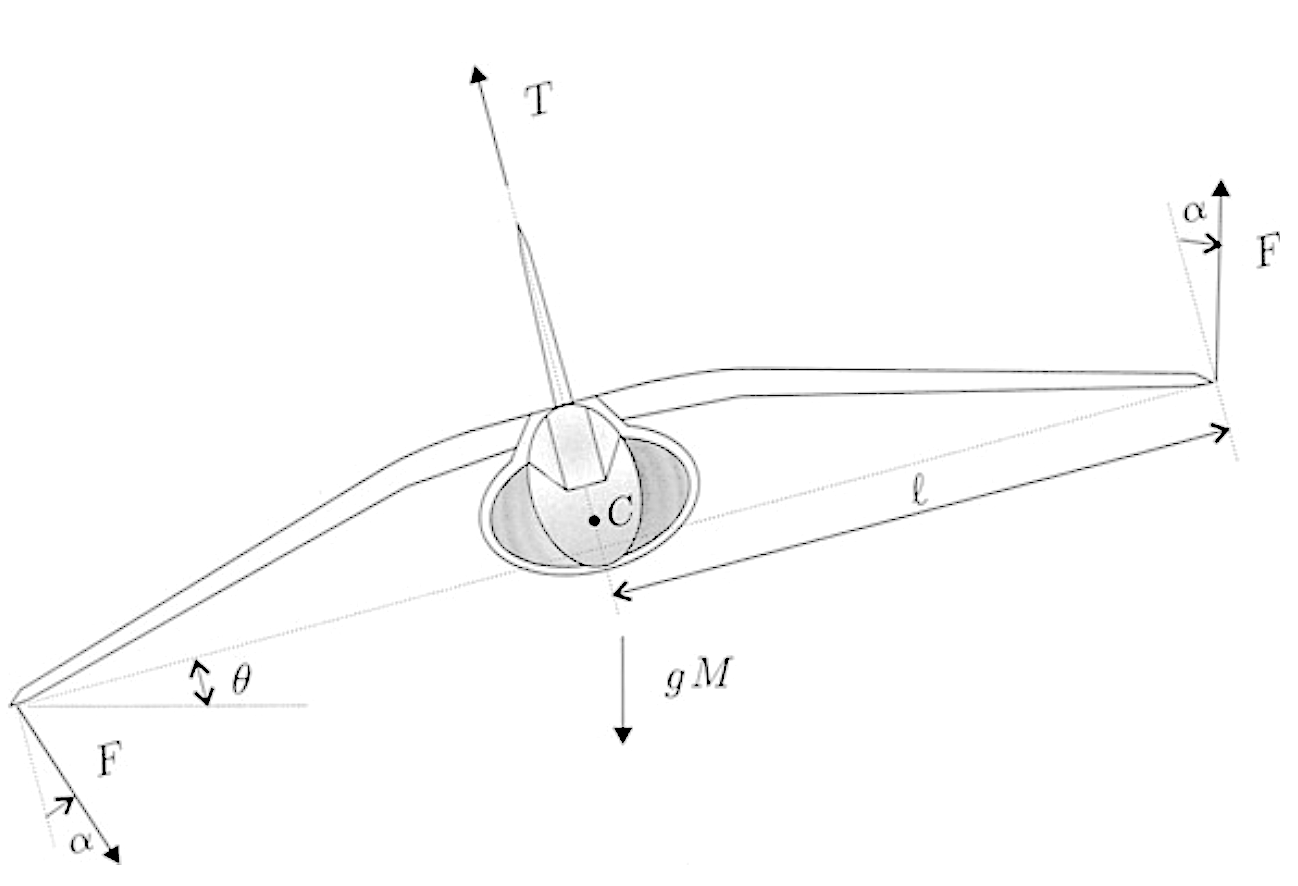
\includegraphics[width=0.8\textwidth]{Figs/Chapter8-9/postprocessing_vtol.png}
	\caption{The vertical takeoff and landing aircraft considered in numerical simulations.}
	\label{FIG:OR-POSTPROCESSING-VERTICAL-TOL}
\end{figure}
%%%%%%%%%%
The proposed regulator reads as follows
\begin{equation}%
   \label{EQ:OR-POST-PROCESSING-OVERALL-REGULATOR}
   \begin{split}
      &
      \begin{cases}
         \dot{\clock} & = 1 \\
         \dot{\im} & = \imfun(\im, \pmu(\im, \id, \alpha, \clock)) + Ge \\
         \dot{\obs}_1 & = \obs_2 - m_1 \obsgain(\obs_1 - \im_d) \\
         \dot{\obs}_2 & = \dot{\pmu}(\im, \id, \alpha, \clock) - m_2 \obsgain^2 (\obs_1 - \im_d) \\
         \dot{\id} & = 0 \\
      \end{cases} \\
      & \lp \im, \obs_1, \obs_2, \id, \clock \rp \in \CC, \\
      &
      \begin{cases}
         \clock^{+} & = 0 \\
         \im^{+} & = \im \\
         \obs_1^{+} & = \obs_1 \\
         \obs_2^{+} & = \obs_2 \\
         \id^{+} & = \lp S \otimes I_{p}\rp \id + \lp B \otimes I_{p}\rp \begin{bmatrix} \im & \obs_2 & \clock \end{bmatrix}\T \\
      \end{cases} \\
      & \lp \im, \obs_1, \obs_2, \id, \clock \rp \in \DD, \\
   \end{split}
\end{equation}
in which $\alpha = \gamma \lp \id \rp \in \R^{N \times N}$, $p = d\dd{\ee} + \dd{\ee} + 1$,
$\lp \obs_1, \obs_2 \rp \in \R^{\dd{\ee}} \times \R^{\dd{\ee}}$, and $\id \in \R^{\dd{\id}}$ with $\dd{\id} = pN$.
The matrices $S \in \R^{N \times N}$ and $B \in \R^{N}$ have the ``shift'' form
\begin{equation*}
   \begin{matrix}
      S = 
      \begin{pmatrix}
         0_{(N-1) \times 1} & I_{N-1} \\
         0 & 0_{1 \times (N-1)}
      \end{pmatrix}, &
      B = 
      \begin{pmatrix}
         0_{(N-1) \times 1} \\ 1
      \end{pmatrix},
   \end{matrix}
\end{equation*}
while $\imfun$ and $G$ have the same structure described by Equation~\eqref{EQ:POSTP-INTERNAL-MODEL},
$\CC = \{ \lp \im, \obs_1, \obs_2, \id, \clock \rp \in \R^{d\dd{\ee}} \times \R^{\dd{\ee}} \times \R^{\dd{\ee}} \times \idset \times \R_{\ge 0} : \pvar \lp \im, \id, \alpha, \clock \rp \le \pvar_{\text{thr}} \}$
represents the flow set, and
$\DD = \{ \lp \im, \obs_1, \obs_2, \id, \clock \rp \in \R^{d\dd{\ee}} \times \R^{\dd{\ee}} \times \R^{\dd{\ee}} \times \idset \times \R_{\ge 0} : \pvar \lp \im, \id, \alpha, \clock \rp \ge \pvar_{\text{thr}} \}$
is the jump set, with $\pvar_{\text{thr}}$ arbitrary. The functions $\pmu \lp \im, \id, \alpha, \clock \rp$ and $\pvar \lp \im, \id, \alpha, \clock \rp$
represent the a posteriori GP estimated mean and variance after the collection of $N$ samples, and $\idset \subseteq \R^{N \dd{\id}}$.
The proposed regulator is composed of \textit{(a)} a purely continuous-time subsystem $\lp \im, \obs_1, \obs_2 \rp$ whose dynamics depends
on $\id$ and $\alpha$ that are constant during flow, \textit{(b)} a purely discrete-time subsystem $\id$ updated ad each jump time,
and \textit{(c)} a hybrid clock $\clock$. Note that, due to the definition of the sets $\CC$ and $\DD$ the jumping law is not directly
related to the clock variable $\clock$, thus at the moment it is not clear if~\eqref{EQ:OR-POST-PROCESSING-OVERALL-REGULATOR} suffers from
\textit{zeno} or \textit{chattering} issues.
The subsystem $\im$ plays the role of internal model unit, and it is taken of the same form as~\eqref{EQ:POSTP-INTERNAL-MODEL}.
The subsystem $\lp \obs_1, \obs_2 \rp$ plays the role of \textit{observer} of the quantity $\dot{\im}_d$ required to build the 
data-set and not directly available. The dynamic equation of $\lp \dot{\obs}_1, \dot{\obs}_2 \rp$ follows the canonical high-gain construction
with the coefficients $m_1, m_2 > 0$ arbitrary and $\obsgain > 0$ left as a design parameter.
The quantities $\lp \obs_2, \im \rp$ act as proxy for the ideal $\lp \dot{\im}_d\s, \im\s \rp$ required to build an approximation of $\imfunsingle\s$;
$\lp \obs_2, \im \rp$ are thus feeded to the discrete-time GP regressor represented by the subsystem $\id$ and by the properly defined
functions $\lp \pmu, \pvar, \gamma \rp$. In particular, denoting $\cvar = \col{\im, \clock}$, the latter functions read as
\begin{equation*}
   \begin{split}
      \pmu \lp \cvar \rp & = \kv \lp \cvar \rp\T \gamma \lp \id \rp \boldsymbol{\obs_2}, \\
      \pvar \lp \cvar \rp & = \kf \lp \cvar, \cvar \rp - \kv \lp \cvar \rp\T \gamma \lp \id\rp \kv \lp \cvar \rp, \\
      \gamma \lp \id \rp & = \lp \km + \nn I_{N} \rp^{-1},
   \end{split}
\end{equation*}
where $\kv$ and $\km$ are defined as in~\secref{SEC:OR-POST-PROCESSING-GAUSSIAN-INFERENCE},
with the only differency that the kernel function $\kf$ has been enhanced by adding a dependency from $\clock$.
In this context, Equation~\eqref{EQ:OR-POST-PROCESSING-EXPONENTIAL-KERNEL} takes the form
\begin{equation*}
   \begin{split}
      \kf \lp \cvar_i, \cvar_j \rp = \pvar_p \exp & \lp - \lp \im_i - \im_j \rp\T \Lambda^{-1} \lp \im_i - \im_j \rp \rp \\
        & \exp \lp -\sum_{k = \min(i, j)}^{\max(i, j)} \norm{\frac{\clock_k}{2 \lambda_{\clock}}} \rp \text{if } \cvar_i, \cvar_j \in \bcvar,
   \end{split}
\end{equation*}
\begin{equation}%
   \label{EQ:OR-POST-PROCESSING-EXPONENTIAL-KERNEL-TIME-2}
   \begin{split}
      \kf(\cvar, \cvar_j) = \pvar_p \exp & \lp - \lp \im - \im_j \rp\T \Lambda^{-1} \lp \im - \im_j \rp \rp \\
        & \exp \lp - \frac{\clock}{2 \lambda_{\clock}^2} + \sum_{k = j}^{m} \norm{\frac{\clock_k}{2 \lambda_{\clock}}} \rp \text{if } \cvar \notin \bcvar, \cvar_j \in \bcvar,
   \end{split}
\end{equation}
where $\lambda_{\clock}$ is a parameter to be tuned and the quantity $\lp \bcvar, \boldsymbol{\obs_2} \rp$ represents the data-set
constructed as discussed in~\secref{SEC:OR-POST-PROCESSING-GAUSSIAN-INFERENCE} extended with the sampled clock $\clock$,
and stored, as a state variable, inside the shift register $\id$.
The addition of the clock as independent variable inside the GP regression is the key to obtain a good estimation of $\imfunsingle$ starting from
the noisy proxy $\lp \obs_2, \im \rp$. This choice is motivated by the fact that the introduction of $\clock$ allows us to shape $\pmu$
through the parameter $\lambda_{\clock}$ whose inverse value can be interpreted as a \textit{forgetting factor}, commonly used in identification.

The design parameters $\lp g, l, \delta, \rho \rp$ in~\eqref{EQ:OR-POST-PROCESSING-OVERALL-REGULATOR} can be chosen so that the closed-loop
system has an asymptotic regulation error bounded by a function of the best attainable prediction, namely
\begin{equation*}
   \lim_{t \to \infty} \sup \norm{\ee(t)} = c_{\ee} \lim_{t \to \infty} \sup \norm{\dot{\im}_d\s(t) - \pmu(\im\s(t))},
\end{equation*}
with $c_{\ee}$ constant that depends on the chosen parameters.
Such a results directly follows from the adaptation of the arguments reported by~\cite{bin2019class} and~\cite{bin2020approximate}
in the specific case in which~\eqref{EQ:OR-POST-PROCESSING-OVERALL-REGULATOR} satisfies a set of properties known as \textit{identifier requirements}.
The following results are instrumental to verify that the proposed regulator fits inside the same framework of~\cite{bin2019class} and~\cite{bin2020approximate}.
\begin{lemma}%
   \label{LEMMA:DWELL-TIME}
   Let Assumptions~\ref{ASSUM:INTERNAL-MODEL},~\ref{ASSUM:MU-CONTINUOUS-BOUNDED}, and~\ref{ASSUM:K-CONTINUOUS-BOUNDED} hold.
   Moreover, suppose that the chosen $\pvar_{\text{thr}}$ satisfies
   \begin{equation}%
      \label{EQ:OR-POSTP-SIGMA-CONDITION}
      \frac{\np \nn}{\np + \nn} < \pvar_{\text{thr}} < \np,
   \end{equation}
   then any solution $\lp \im, \obs_1, \obs_2, \id, \clock \rp$ of~\eqref{EQ:OR-POST-PROCESSING-OVERALL-REGULATOR} originating from the set
   $\chi_0 = \{ \lp \im, \obs_1, \obs_2, \id, \clock \rp \in \R^{d\dd{\ee}} \times \R^{\dd{\ee}} \times \R^{\dd{\ee}} \times \idset \times \R_{\ge 0} : \clock = 0\}$
   satisfies a dwell time condition in the sense of~\cite{hespanha1999stability}, and a reverse dwell time condition in
   the sense of~\cite{hespanha2005input}.
\end{lemma}
\begin{proof}
   Using the same arguments proposed by~\cite{hespanha2005input}, we shape the proof to show the existence of $\overline{\text{T}}$ and $\underline{\text{T}}$
   such that $\CC \subseteq \{ \lp \im, \obs_1, \obs_2, \id, \clock \rp \in \R^{d\dd{\ee}} \times \R^{\dd{\ee}} \times \idset \times \R^{mp} \times \R_{\ge 0} : 0 \le \clock \le \overline{\text{T}} \}$
   and $\DD \subseteq \{ \lp \im, \obs_1, \obs_2, \id, \clock \rp \in \R^{d\dd{\ee}} \times \R^{\dd{\ee}} \times \idset \times \R^{mp} \times \R_{\ge 0} : \underline{\text{T}} \le \clock \le \overline{\text{T}} \}$.
   First note that, in view of~\assumptionref{ASSUM:INTERNAL-MODEL}, from the definition of kernel in~\eqref{EQ:OR-POST-PROCESSING-EXPONENTIAL-KERNEL-TIME-2},
   the value of $\pvar \lp \im, \id, \alpha, \clock \rp$ reaches $\np$ as long as $t$ goes to infinty, i.e.
   \begin{equation}%
      \label{EQ:OR-POSTP-SIGMA-LIMIT}
      \lim_{t \to \infty} \pvar \lp \im(t), \id(t), \alpha(t), \clock(t) \rp = \np.
   \end{equation}
   Recalling $\cvar = \col{\im, \clock}$, then the flow and jump dynamics of $\pvar$ are described by
   \begin{equation}%
      \label{EQ:OR-POSTP-SIGMA-FLOW}
      \begin{split}
         \dot{\lp \pvar\rp} & = \dot{\cvar}\T \lp \frac{d \kf \lp \cvar, \cvar \rp}{d \cvar} - 2 \frac{d \kv(\cvar)}{d \cvar}\T \gamma \lp \id \rp \kv \lp \cvar \rp \rp \\
         & = - 2 \dot{\cvar}\T \frac{d \kv \lp \cvar \rp}{d \cvar}\T \gamma \lp \id \rp \kv \lp \cvar \rp,
      \end{split}
   \end{equation}
   when $\lp \im, \obs_1, \obs_2, \id, \clock\rp \in \CC$, and
   \begin{equation}%
      \label{EQ:OR-POSTP-SIGMA-JUMP}
      \lp \pvar \rp^+ = \kf \lp \cvar^+, \cvar^+ \rp - \kv \lp \cvar^+ \rp \gamma \lp \id^+ \rp \kv \lp \cvar^+ \rp,
   \end{equation}
   when $\lp \im, \obs_1, \obs_2, \id, \clock\rp \in \DD$.
   The existence of $\overline{\text{T}}$ follows from~\eqref{EQ:OR-POSTP-SIGMA-LIMIT} and the second inequality of~\eqref{EQ:OR-POSTP-SIGMA-CONDITION},
   in particular by choosing $\pvar_{\text{thr}} < \np$, since $\pvar \to_{\clock \to \infty} \np$, there exists a real value $\overline{\text{T}}$
   such that $\pvar \ge \pvar_{\text{thr}}$ for any $\clock \ge \overline{\text{T}}$. This ensures persistency of jump intervals.
   Consider now Equations~\eqref{EQ:OR-POSTP-SIGMA-FLOW} and~\eqref{EQ:OR-POSTP-SIGMA-JUMP}, the flow dynamics $\dot{\lp \pvar \rp}$ results to be a continous function
   being it a product of Lipschitz functions (Assumptions~\ref{ASSUM:INTERNAL-MODEL},~\ref{ASSUM:MU-CONTINUOUS-BOUNDED},~\ref{ASSUM:K-CONTINUOUS-BOUNDED}).
   Moreover, its norm can be upper bounded as
   \begin{equation*}
      \norm{\dot{\lp \pvar\rp}} \le 2 \norm{\dot{\cvar}} \norm{\frac{d \kv \lp \cvar \rp}{d \cvar}} \norm{\gamma \lp \id \rp} \norm{\kv \lp \cvar \rp},
   \end{equation*}
   with $\dot{\cvar} = \lps \im_2, \dots, \im_d, \imfunsingle \lp \im \rp, 1 \rps\T$.
   Since during flow the function $\kf$ takes the form of~\eqref{EQ:OR-POST-PROCESSING-EXPONENTIAL-KERNEL-TIME-2}, rewriting the latter as
   \begin{equation*}
      \kf \lp \cvar, \cvar_j \rp = \np \exp\lp -\lp \cvar-\cvar_j \rp\T \bar{\Lambda}^{-1} \lp \cvar-\cvar_j \rp\rp,
   \end{equation*}
   the quantity 
   \begin{equation*}
      \frac{d \kv \lp \cvar \rp}{d \cvar} =
      \begin{bmatrix}
		-\kf \lp \cvar, \cvar^1 \rp \bar{\Lambda}^{-1} \lp \cvar - \cvar^1 \rp \\
		-\kf \lp \cvar, \cvar^2 \rp \bar{\Lambda}^{-1} \lp \cvar - \cvar^2 \rp \\
		\vdots \\
		-\kf \lp \cvar, \cvar^m \rp \bar{\Lambda}^{-1} \lp \cvar - \cvar^m \rp
      \end{bmatrix},
   \end{equation*}
   where $\cvar^i$ denotes the $i$th training point stored inside $\id$, and with $\bar{\Lambda}$ properly defined.
   \assumptionref{ASSUM:INTERNAL-MODEL} ensures $\norm{\dot{\cvar}} \le l_{\cvar}$, with $l_{\cvar}$ dependent on the chosen $H\s$,
   while~\assumptionref{ASSUM:K-CONTINUOUS-BOUNDED} ensures boundedness of $\gamma \lp \id \rp$ and $\kv \lp \cvar \rp$, namely
   \begin{equation*}
      \begin{matrix}
         \norm{\gamma \lp \id \rp} \le l_{\gamma}, &
         \norm{\kv \lp \cvar \rp} \le l_{k}
      \end{matrix}.
   \end{equation*}
   From the previous arguments follows that $\norm{d \kv \lp \cvar \rp / d \cvar} \le l_{dk}$, yielding to
   $\norm{\dot{\pvar}} \le l_{\pvar}$ with $l_{\pvar} = l_{\cvar}l_{dk}l_{\gamma}l_{k}$.
   Note that the bound $l_{\pvar}$ does not depend neither on the chosen regulator parameters, nor on the initial conditions.
   Consider now the jump dynamics, under the~\assumptionref{ASSUM:K-CONTINUOUS-BOUNDED} of Lipschitz continuous kernel, we can explicitly derive an upper bound on
   the value of $\lp \pvar \rp^+$ at each jump (see~\cite[Theorem 1]{lederer2021uniform})
   \begin{equation*}
    	\begin{split}
			\lp \pvar\rp^+ \le \Big[ \big| \BB \lp \bar{\cvar} \rp & \big| \lp \kf \lp \cvar\s, \cvar\s \rp + 2L_{k} \varrho \rp + \nn \Big]^{-1} \\
			& \Big[ \lp 2lb \big( \kf\lp\cvar^+, \cvar^+ \rp + \kf \lp \cvar\s, \cvar^+ \rp\rp \\ 
			& - L_{k}^2 \varrho^2\big) \big|\BB\lp\cvar\s\rp\big| + \nn \kf\lp\cvar^+, \cvar^+\rp\Big],
    	\end{split}
   \end{equation*}
   where $\BB \lp \cvar\s \rp$ denotes the training data set restricted to a ball around $\cvar\s$ with radius $\varrho \in \R$.
   In our specific case $\cvar\s = \cvar^+$, thus the aforementioned relation boils down to
   \begin{equation*}
		\lp \pvar\rp^+ \le \frac{\lp 4L_k \varrho \np - L_k^2 \varrho^2\rp m_{\BB \lp \cvar\s \rp} + \nn \np}{\lp \np + L_k \varrho\rp m_{\BB \lp \cvar\s \rp} + \nn}
   \end{equation*}
   with $\varrho \le \np / L_k$ and $m_{\BB\lp\cvar\s\rp} \le m$ is the cadinality of $\BB\lp\cvar\s\rp$.
   Clearly, the worst case scenario is represented by the case in wich $\BB\lp\cvar\s\rp$ cannot embrace any training points, thus when $\varrho = 0$.
   In this particular case we get
   \begin{equation*}
      \lp \pvar\rp^+ \le \frac{\nn \np}{\np + \nn} < \pvar_{\text{thr}}.
   \end{equation*}
   Finally, the existence of $\underline{\text{T}}$ follows from the fact that the flow dynamics~\eqref{EQ:OR-POSTP-SIGMA-FLOW} is continuous
   with upper bounded norm and its initial condition, at each jump time, is lower than the chosen threshold $\pvar_{\text{thr}}$.
   This ensures persistency of flow intervals.
\end{proof}
\begin{lemma}
   Consider the hybrid subsystem
   \begin{equation}%
      \label{EQ:OP-POSTP-HYBRID-SUBSYSTEM}
      \begin{split}
         &
         \begin{cases}
            \dot{\clock} & = 1 \\
            \dot{\im} & = \imfun \lp \im, \pmu \lp \im, \id, \alpha, \clock \rp \rp + Ge \\
            \dot{\id} & = 0 \\
         \end{cases} \\
         & \lp \im, \id, \clock \rp \in \CC, \\
         &
         \begin{cases}
            \clock^{+} & = 0 \\
            \im^{+} & = \im \\
            \id^{+} & = \lp S \otimes I_{p}\rp \id + \lp B \otimes I_{p}\rp \\ 
            & \hspace{1.5cm} \begin{bmatrix} \im+\delta_{\im_{1:d-1}} & \im_d+\delta_{\im_d} & \clock \end{bmatrix}\T \\
         \end{cases} \\
         & \lp \im, \id, \clock \rp \in \DD, \\
      \end{split}
   \end{equation}
   with $\CC$ and $\DD$ defined as above and $\delta_{\im} = \lp \delta_{\im_{1:d-1}}, \delta_{\im_d} \rp \in \R^{d\dd{\ee}}$ hybrid input.
   Let Assumptions~\ref{ASSUM:MU-CONTINUOUS-BOUNDED} and~\ref{ASSUM:K-CONTINUOUS-BOUNDED}, and Lemma~\ref{LEMMA:DWELL-TIME} hold, then the tuple $\lp \idset, \pmu, \gamma, \alpha\rp$
   satisfies the identifier requirements~\cite{bin2020approximate} relative to $\loss$, namely there exists a compact set $S\s \subset \idset$, $\beta_{\id} \in \KL$,
   a Lipschitz function $\rho_{\id} \in \KK$, and for each solution $\lp \ww, \xx, \im, \clock \rp$ to
   Equations~\eqref{EQ:GENERAL-EXOSYSTEM},~\eqref{EQ:POSTP-FRAMEWORK}, and~\eqref{EQ:POSTP-INTERNAL-MODEL},
   a hybrid arc $\id\s: \text{dom}\lp \ww, \xx, \im, \clock\rp \mapsto \idset$ and a $j\s \in \N$ such that $\lp \clock, \im, \id\s, d \rp$ with $\delta_{\im} = 0$
   is a solution pair to~\eqref{EQ:OP-POSTP-HYBRID-SUBSYSTEM} satisfying $\id\s(j) \in S\s$ for all $j \ge j\s$, and the following holds:
   \begin{enumerate}
      \item \textit{\textbf{Optimality:}}
      For all $j \ge j\s$, the function $\pmu\s(\cdot) = \pmu\lp \im, \id\s, \gamma \lp \id\s \rp, \clock \rp$ satisfies
      \begin{equation*}
        \pmu\s_j(\cdot) \in \arg \min \loss_j.
      \end{equation*}
      \item \textit{\textbf{Stability:}}
      For every hybrid input $\delta_{\im}$, every solution pair $\lp \im, \id, \clock, \delta \rp$ of the hybrid subsystem~\eqref{EQ:OP-POSTP-HYBRID-SUBSYSTEM}
      satisfies for all $j \in \text{Jmp}\lp \im, \id, \clock \rp$
      \begin{equation*}
        \lb \id(j) - \id\s(j) \rb \le \max \{ \beta_{\id}(\lb \id(0) - \id\s(0) \rb,j), \rho_{\id}(\lb \delta_{\im} \rb_j) \}.
      \end{equation*}
      \item \textit{\textbf{Regularity:}}
      The map $\pmu(\cdot)$ is Lipschitz and differentiable with a locally Lipschitz derivative.
   \end{enumerate}
\end{lemma}
The proof of the latter lemma directly follows from the same arguments proposed by~\cite[Proposition 2]{bin2020approximate}.

\subsection{Numerical Simulations}%
\label{SEC:OR-POSTP-NUMERICAL-SIMULATIONS}
%%%%%%%%%%
\begin{figure}[!t]
	\centering
	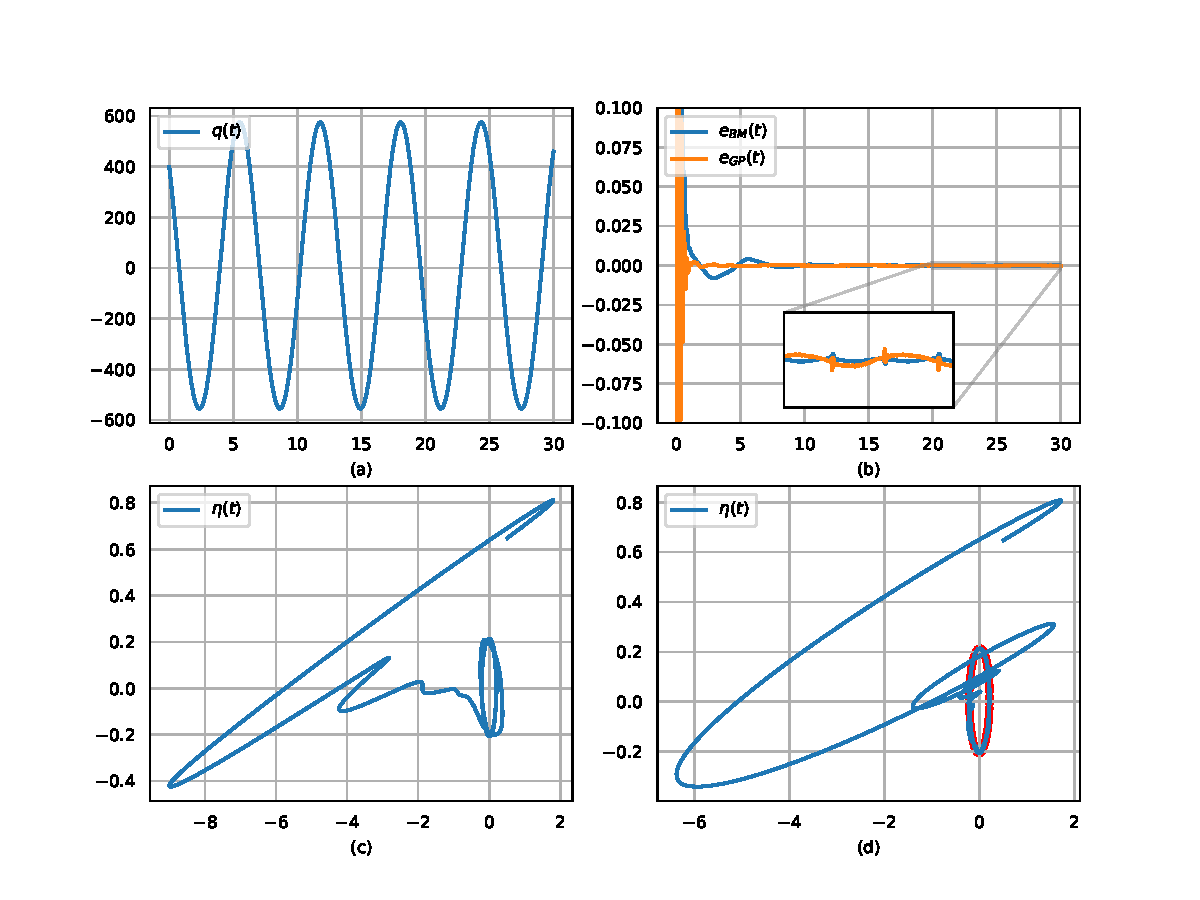
\includegraphics[width=1.\textwidth]{Figs/Chapter8-9/postprocessing_lin_example.pdf}
	\caption{Results obtained comparing our approach $(e_{GP})$ versus~\cite{bin2019class} $(e_{BM})$ when the exogenous disturbance $d(\ww)$ is generated by~\eqref{EQ:OR-POSTP-EXOSYSTEM-1}.
	In both cases, the used regulator parameters are the same reported in~\tabref{TAB:POSTP-REGULATOR-SIMULATION-PARAMETERS}.
	In the figure, image $(a)$ depicts the injected noise, $(b)$ compares the behavior of the regulation errors, while $(c)$ and $(d)$ shows the dynamics of $(\im_1, \im_2)$
	along the experiments in which the Bin-Marconi regulator~\cite{bin2019class} and ours is applied, respectively. In figure $(c)$ the used samples $(\id)$ during the last
	flow interval are shown as green dots. The reported quantities are plotted with respect to the time in seconds (abscissa).}
	\label{FIG:OR-POSTPROCESSING-LIN-RESULTS}
\end{figure}
%%%%%%%%%%
%%%%%%%%%%
\begin{figure}[!t]
	\centering
	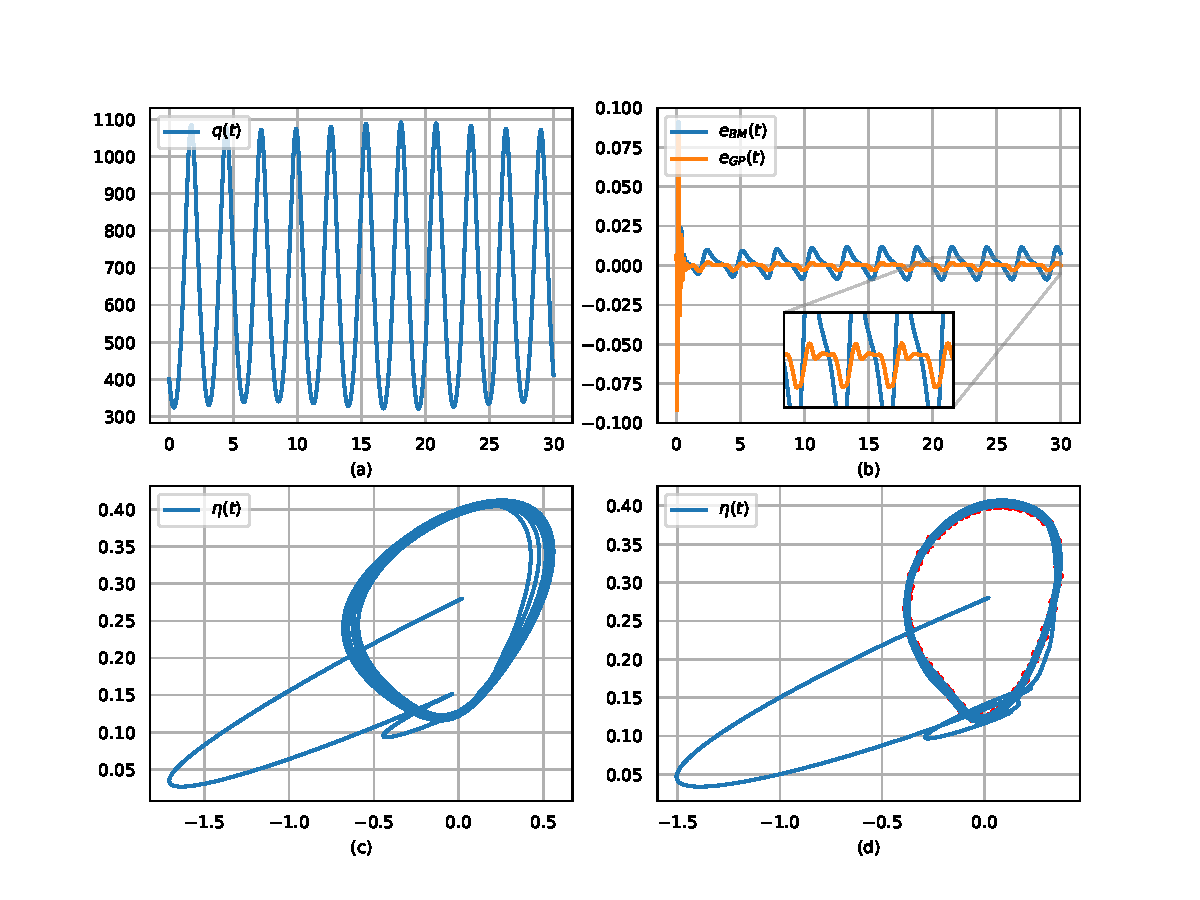
\includegraphics[width=1.\textwidth]{Figs/Chapter8-9/postprocessing_pow_example.pdf}
	\caption{Results obtained comparing our approach $(e_{GP})$ versus~\cite{bin2019class} $(e_{BM})$ when the exogenous disturbance $d(\ww)$ is generated by~\eqref{EQ:OR-POSTP-EXOSYSTEM-2}.
	For a comprehensive explanation of Figures $(a)$, $(b)$, $(c)$, and $(d)$ please refer to~\figref{FIG:OR-POSTPROCESSING-LIN-RESULTS}. The reported quantities are plotted with respect to the time in seconds (abscissa).}
	\label{FIG:OR-POSTPROCESSING-POW-RESULTS}
\end{figure}
%%%%%%%%%%
%%%%%%%%%%
\begin{figure}[!t]
	\centering
	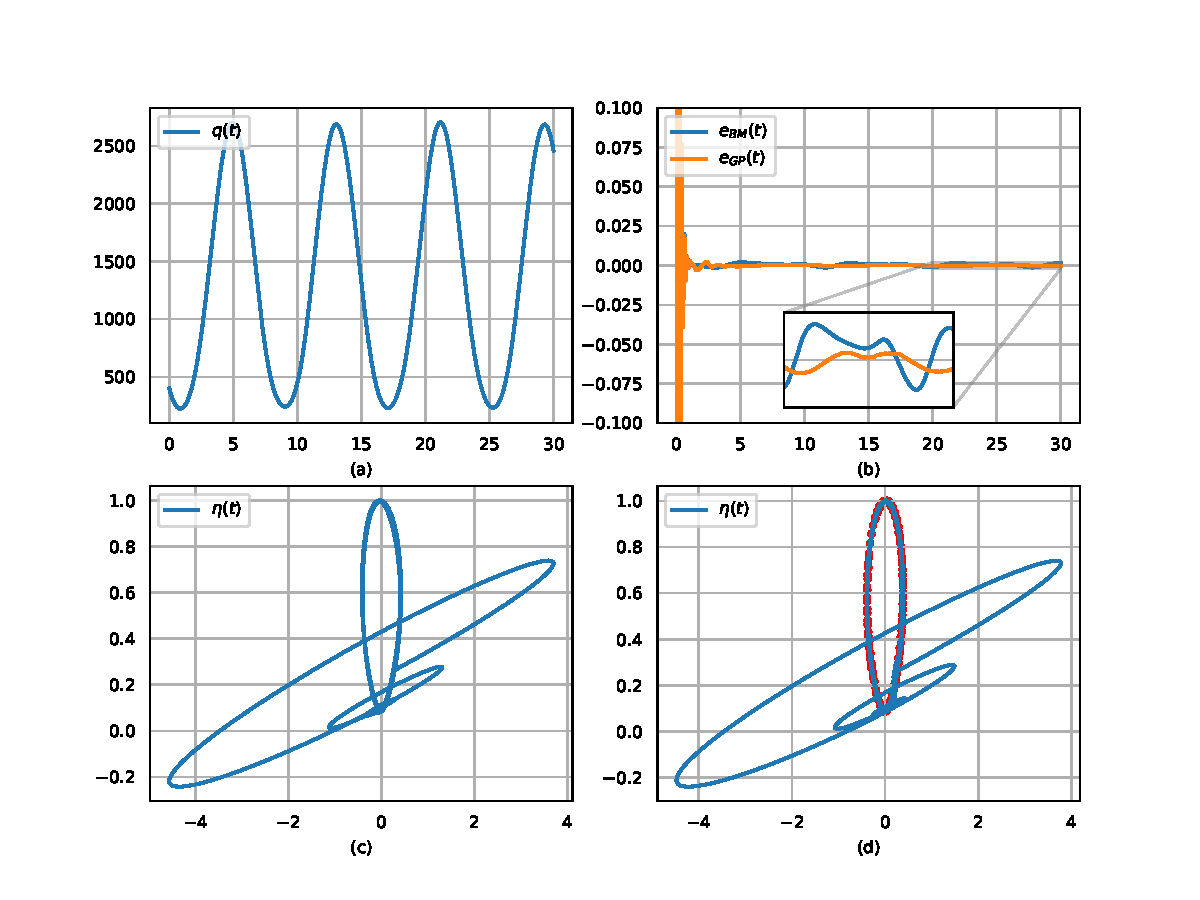
\includegraphics[width=1.\textwidth]{Figs/Chapter8-9/postprocessing_atan_example.pdf}
	\caption{Results obtained comparing our approach $(e_{GP})$ versus~\cite{bin2019class} $(e_{BM})$ when the exogenous disturbance $d(\ww)$ is generated by~\eqref{EQ:OR-POSTP-EXOSYSTEM-3}.
	For a comprehensive explanation of Figures $(a)$, $(b)$, $(c)$, and $(d)$ please refer to~\figref{FIG:OR-POSTPROCESSING-LIN-RESULTS}. The reported quantities are plotted with respect to the time in seconds (abscissa).}
	\label{FIG:OR-POSTPROCESSING-ATAN-RESULTS}
\end{figure}
%%%%%%%%%%
\begin{table}[b!]
	\centering
	\begin{tabular}{||c|c|c|c|c|c|c||}
		\hline
		\hline
		$N$ & $\lambda_{\im_1}$ &  $\lambda_{\im_2}$ & $\lambda_{\clock}$ & $\np$ & $\nn$ & $\pvar_{\text{thr}}$ \\
		\hline
		$100$ & $0.1$ & $0.1$ & $2$ & $1$ & $0.01$ & $0.1$\\
		\hline
		\hline
	\end{tabular}
	\caption{Gaussian process parameters used in simulations.}%
	\label{TAB:POSTP-GP-SIMULATION-PARAMETERS}
\end{table}
\begin{table}[b!]
	\centering
	\begin{tabular}{||c|c|c|c|c|c|c|c||}
		\hline
		\hline
		$\lp c_1, c_2, c_3\rp$ & $l$ & $\delta$ & $\LL$  & $\lp h_1, h_2\rp$ & $g$ & $\lp m_1, m_2\rp$ & $\rho$ \\
		\hline
		$\lp 15, 75, 125\rp$ & $250$ & $150$ & $20$ & $\lp 15, 70\rp$ & $2$ & $\lp 20, 20\rp$ & $2$ \\
		\hline
		\hline
	\end{tabular}
	\caption{Regulator parameters used in simulations.}%
	\label{TAB:POSTP-REGULATOR-SIMULATION-PARAMETERS}
\end{table}
\begin{table}[b!]
	\centering
	\begin{tabular}{||c|c|c|c||}
		\hline
		\hline
		$M$ & $J$ & $\boldsymbol{l}$ & $\boldsymbol{g}$ \\
		\hline
		$5\cdot 10^4$ & $1.25 \cdot 10^4$ & $2$ & $9.81$ \\
		\hline
		\hline
	\end{tabular}
	\caption{Model parameters used in simulations.}%
	\label{TAB:POSTP-MODEL-SIMULATION-PARAMETERS}
\end{table}
We consider, as a testbed, the problem of regulation the lateral $\lp y_1, y_2 \rp$ and angular $\lp \theta_1, \theta_2 \rp$
dynamics of a Vertical-TakeOff-and-Landing (VTOL) aircraft~\cite{isidori2003robust} subjected to lateral forces
produced by the wind denoted by $d(w)$. A graphical representation of the considered system is reported in~\figref{FIG:OR-POSTPROCESSING-VERTICAL-TOL}.
The VTOL dynamics reads as
\begin{equation}%
   \label{EQ:OR-POSTP-VTOL-DYNAMICS}
   \begin{matrix}
      \begin{split}
        \dot{y}_1 & = y_2,  \\ \dot{y}_2 & = d(\ww) - \boldsymbol{g} \tan(\theta_1) + v,
      \end{split} & 
      \begin{split}
        \dot{\theta}_1 & = \theta_2, \\ \dot{\theta}_2 & = 2\boldsymbol{l}J^{-1}\uu,
      \end{split}
   \end{matrix}
\end{equation}
where $M>0$ and $J>0$ are the aircraft mass and inertia respectively, while $\boldsymbol{l}>0$ represents the wings lenght and $\boldsymbol{g} > 0$ the
gravitational constant. The input $\uu$ is the force $\lp F \rp$ on the wingtips, $v$ is a vanishing input taking into
account the (controlled) vertical dynamics (not considered here), and $d(\ww) := M^{-1}d_0(\ww)$, with $d_0(\ww)$ that is
the lateral force produced by the wind. Considering as regulation error the aircraft lateral position $\lp \ee = y_1\rp$, the control
objective is to remove the wind disturbance out from the lateral dynamics.
Let $\ww(t)$ be generated by an exosystem of the form~\eqref{EQ:GENERAL-EXOSYSTEM} and consider the following change of coordinates
\begin{equation*}
   \begin{matrix}
      \begin{split}
        \chi_1 & = y_1, \\ \chi_2 & = y_2,
      \end{split} &
      \begin{split}
        \chi_3 & = d(\ww) + \boldsymbol{g} \tan(\theta_1), \\ \zeta & = L_s d(\ww) - {\boldsymbol{g} \theta_2}/{\cos(\theta_1)}.
      \end{split}
   \end{matrix}
\end{equation*}
In the new coordinates, letting $\xx = \col{\chi, \zeta}$, the system~\eqref{EQ:OR-POSTP-VTOL-DYNAMICS} reads as follow
\begin{equation}%
   \label{EQ:OR-POSTP-NEW-VTOL-SYSTEM}
   \begin{matrix}
      \begin{split}
         \dot{\chi}_1 & = \chi_2, \\
         \dot{\chi}_2 & = \chi_3,
      \end{split} &
      \begin{split}
         \dot{\chi}_3 & = \zeta, \\
      \dot{\zeta} & = \qfun(\ww,\xx) + \bfun(\ww,\xx)\uu,
      \end{split}
   \end{matrix}
\end{equation}
with $\qfun(\ww,\xx)$ and $\bfun(\ww,\xx)$ given by
\begin{equation*}
   \begin{split}
      \qfun(\ww,\xx) = L_s^2 d(\ww) - & \frac{1}{\boldsymbol{g}} \lp L_s d(\ww) - \zeta\rp^2 \\
      & \sin\lp 2 \tan^{-1}\lp \frac{d(\ww) - \chi_3}{\boldsymbol{g}}\rp\rp,
   \end{split}
\end{equation*}
\begin{equation*}
   \bfun(\ww,\xx) = -2\boldsymbol{g}\boldsymbol{l}J^{-1} \cos\lp \tan^{-1}\lp \frac{d(\ww) - \chi_3}{\boldsymbol{g}}\rp\rp^{-2}.
\end{equation*}
The system~\eqref{EQ:OR-POSTP-NEW-VTOL-SYSTEM} is in the form~\eqref{EQ:POSTP-FRAMEWORK} with~\assumptionref{ASSUM:REGULATOR-EQUATIONS} trivially fulfilled, since
the $\zz$ dynamics is absent, by $\xx\s = 0$ and $\uu\s = (\boldsymbol{g}L_s^2d(\ww) - 2d(\ww)(\boldsymbol{g}^2 + d(\ww)^2)(L_sd(\ww))^2)/2\boldsymbol{l}J^{-1}(\boldsymbol{g}^2 + d(\ww)^2)$,
and~\assumptionref{ASSUM:STABILIZABILITY-ASSUMPTION} fulfilled on each compact set with $\LL$ a negative number.
With $\lp c_1,c_2,c_3 \rp$ the coefficients of a Hurwitz polynomial and $\delta,l > 0$ design parameters, we fix the control law as
\begin{equation*}
   \begin{split}
      \uu = \LL\Big[ c_1 & l \delta^3 (y_1 + \im_1) + c_2  l \delta^2 y_2 \\ 
        & + c_3 l \delta (-\boldsymbol{g} \tan(\theta_1)) + l(-\boldsymbol{g} \theta_2 / \cos^2(\theta_1)) \Big].
   \end{split}
\end{equation*}
Figures~\ref{FIG:OR-POSTPROCESSING-LIN-RESULTS},~\ref{FIG:OR-POSTPROCESSING-POW-RESULTS}, and~\ref{FIG:OR-POSTPROCESSING-ATAN-RESULTS}
report the obtained results when the aircraft is perturbed with a lateral disturbance $d(w) = (2(10^7\ww_1) + 10^6\ww_3)/M$, where
$\ww_1$ and $\ww_3$ are the states of three different exosystems. In particular, in~\figref{FIG:OR-POSTPROCESSING-LIN-RESULTS}, $\wfun(\ww)$ reads as
\begin{equation}%
   \label{EQ:OR-POSTP-EXOSYSTEM-1}
   \begin{matrix}
      \begin{split}
         \dot{\ww}_1 & = \ww_2, \\
         \dot{\ww}_2 & = -\ww_1, \\
      \end{split} &
      \begin{split}
         \dot{\ww}_3 & = \ww_4, \\
         \dot{\ww}_4 & = -4\ww_3,
      \end{split}
   \end{matrix}
\end{equation}
in~\figref{FIG:OR-POSTPROCESSING-POW-RESULTS}, $\wfun(\ww)$ behaves as
\begin{equation}%
   \label{EQ:OR-POSTP-EXOSYSTEM-2}
   \begin{matrix}
      \begin{split}
         \dot{\ww}_1 & = \ww_2, \\
         \dot{\ww}_2 & = 4\ww_1 - \ww_1^3, \\
      \end{split} &
      \begin{split}
         \dot{\ww}_3 & = \ww_4, \\
         \dot{\ww}_4 & = -4\ww_3,
      \end{split}
   \end{matrix}
\end{equation}
while in~\figref{FIG:OR-POSTPROCESSING-ATAN-RESULTS}, the exosystem is described by
\begin{equation}%
   \label{EQ:OR-POSTP-EXOSYSTEM-3}
   \begin{matrix}
      \begin{split}
         \dot{\ww}_1 & = \ww_2, \\
         \dot{\ww}_2 & = 3\tan^{-1}\lp \ww_1\rp - \ww_1, \\
      \end{split} &
      \begin{split}
         \dot{\ww}_3 & = \ww_4, \\
         \dot{\ww}_4 & = -4\ww_3.
      \end{split}
   \end{matrix}
\end{equation}
In all simulations we exploit the same set of parameters, for both the regulator and the discrete-time identifier.
The adopted parameters are reported in~\tabref{TAB:POSTP-GP-SIMULATION-PARAMETERS},~\tabref{TAB:POSTP-REGULATOR-SIMULATION-PARAMETERS}, and~\tabref{TAB:POSTP-MODEL-SIMULATION-PARAMETERS}.

%----------------------------------------------------------------------------------------
\section{Identification-Based Pre-Processing Internal Model}%
\label{SEC:PREP-ADAPTIVE-INTERNAL-MODEL}
In this section, we recall an adaptive pre-processing internal model design technique for a nonlinear system of the same
kind of~\eqref{EQ:POSTP-FRAMEWORK}. In this second case, we set, without loss of generality, $\zin = 0$, and restrict the
analysis to those systems having an equal number of inputs and regulated outputs $\dd{\uu} = \dd{\ee}$. For seek of clarity,
we report here the reference nonlinear system, with a slightly different notation
\begin{equation}%
   \label{EQ:PREP-FRAMEWORK}
   \begin{split}
      \dot{\zz} &= \zfun \lp \ww, \zz, \ee \rp, \\
      \dot{\ee} &= A\ee + B \lp \qfun \lp \ww, \zz, \ee \rp + \bfun \lp w, \zz, \ee \rp u \rp, \\
      \yy &= C\ee,
   \end{split}
\end{equation}
in which $\zz \in \R^{\dd{\zz}}$ together with the error dynamics $\ee \in \R^{\dd{\ee}}$ represent the overall state of the plant.
The quantities $\uu \in \R^{\dd{\yy}}$ and $\yy \in \R^{\dd{\yy}}$ are the control input and the measured output respectively, while $\ww \in \R^{\dd{\ww}}$ is
an exogenous input, $\zfun : \R^{\dd{w}} \times \R^{\dd{\zz}} \times \R^{\dd{\ee}} \mapsto \R^{\dd{\zz}}$,
$\qfun : \R^{\dd{w}} \times \R^{\dd{\zz}} \times \R^{\dd{\ee}} \mapsto \R^{\dd{\yy}}$, $\bfun : \R^{\dd{\ww}} \times \R^{\dd{\zz}} \times \R^{\dd{\ee}} \mapsto \R^{\dd{\yy} \times \dd{\yy}}$
are continuous functions, and $A$, $B$, and $C$ are defined as
\begin{equation*}
   \begin{matrix}
      A =
      \begin{pmatrix}
         0_{(r-1)\dd{\yy} \times \dd{\yy}} & I_{(r-1)\dd{\yy}} \\
         0_{\dd{\yy} \times \dd{\yy}} & 0_{\dd{\yy} \times (r-1)\dd{\yy}}
      \end{pmatrix}, &
      B =
      \begin{pmatrix}
         0_{(r-1)\dd{\yy} \times \dd{\yy}} \\
         I_{\dd{\yy}}
      \end{pmatrix},
   \end{matrix}
\end{equation*}
\begin{equation*}
   C =
   \begin{pmatrix}
      I_{\dd{\yy}} & 0_{\dd{\yy} \times (r-1)\dd{\yy}}
   \end{pmatrix},
\end{equation*}
The presented regulator is based on the following set of standing assumptions.
\begin{assumption}%
	\label{ASSUM:CONTINUITY-ASSUMPTION}
   The function $\zfun$ is locally Lipschitz and the functions $\qfun$ and $\bfun$ are $\CC^1$ functions, with local Lipschitz derivative.
\end{assumption}
\begin{assumption}%
	\label{ASSUM:REGULATOR-EQUATIONS}
   There exists a $\CC^1$ map $\pi: \CC \subset \R^{\dd{\ww}} \mapsto \R^{\dd{\zz}}$, with $\CC$ an open neighborhood of $\wset$, satisfying
   \begin{equation*}
      L_{\wfun \lp \ww \rp}^{\lp \ww \rp} \pi \lp \ww \rp = \zfun \lp \ww, \pi \lp \ww \rp, 0 \rp,
   \end{equation*} 
   with $L_{\wfun \lp \ww \rp}^{\lp \ww \rp} \pi \lp \ww \rp = \frac{\partial \pi \lp \ww \rp}{\partial \ww} \wfun \lp \ww \rp$,
   such that the system
   \begin{equation*}
      \begin{matrix}
         \dot{\ww} = \wfun \lp \ww \rp, & \dot{\zz} = \zfun \lp \ww, \zz, \ee \rp,
      \end{matrix}
   \end{equation*}
   is Input-to-State Stable (ISS) with respect to the input $\ee$,
   relative to the compact set $\set = \left\{ \lp \ww, \zz \rp \in \wset \times \R^{\dd{\zz}} : \zz = \pi \lp \ww \rp \right\}$.
\end{assumption}
\begin{assumption}%
   \label{ASSUM:STABILIZABILITY-ASSUMPTION}
   There exists a known constant nonsingular matrix $\bs{\bfun} \in \R^{\dd{\yy} \times \dd{\yy}}$ such that the inequality
   \begin{equation*}
    	\norm{(\bfun(\ww, \zz, \ee) - \bs{\bfun})\bs{\bfun}^{-1}} \le 1 - \pmu_0,
   \end{equation*}
   holds for some known scalar $\pmu_0 \in \lp 0, 1 \rp$, and for all
   $\lp \ww, \zz, \ee \rp \in \wset \times \R^{\dd{\zz}} \times \R^{\dd{\ee}}$.
\end{assumption}
\begin{remark}
	Although not necessary (see~\cite{byrnes2003limit}),~\assumptionref{ASSUM:REGULATOR-EQUATIONS} is a minimum-phase assumption 
	customary made in the literature of output regulation (see~\cite{isidori2017lectures},~\cite{pavlov2006uniform}).
	In particular,~\assumptionref{ASSUM:REGULATOR-EQUATIONS} is asking that the zero dynamics
	\begin{equation*}
	   \begin{matrix}
		  \dot{\ww} = \wfun \lp \ww \rp, & \dot{\zz} = \zfun \lp \ww, \zz, 0 \rp,
	   \end{matrix}
	\end{equation*}
	has a steady-state of the kind $\zz = \pi \lp \ww \rp$, compatible with the control objective $\yy = 0$.
	As a consequence, the ideal input $\uu\s$ making the set $\BB = \set \times \{0\}$ invariant for~\eqref{EQ:PREP-FRAMEWORK} reads as
	\begin{equation*}
	   \uu\s \lp \ww, \pi \lp \ww \rp \rp = - \bfun \lp \ww, \pi \lp \ww \rp, 0 \rp^{-1} \qfun \lp \ww, \pi \lp \ww \rp, 0 \rp.
	\end{equation*}
	The ability of the regulator to generate such an input is generally referred to as the \emph{internal model property}.
	With a little abuse of notation, from now on we refer to $ \uu\s \lp \ww, \pi \lp \ww \rp \rp$ with $ \uu\s \lp \ww \rp$.
 \end{remark}
 \begin{remark}
	\assumptionref{ASSUM:STABILIZABILITY-ASSUMPTION} is a stabilizability assumption asking that $\bfun \lp \ww, \zz, \ee \rp$
	is always invertible whatever $\lp \ww, \zz, \ee \rp$ is (see~\cite{wang2017robust}).
	Moreover, the designer is required to have access to an estimate $\bs{\bfun}$ of $\bfun \lp \ww, \zz, \ee \rp$
	which captures enough information about its behavior.
 \end{remark}
In this framework, we now recall two results based on~\cite{marconi2007output} and~\cite[Theorem 1]{bin2020approximate}.
\begin{lemma}%
   \label{LEMMA:LUMBERGER-INTERNAL-MODEL}
   Let previous assumptions hold and let $\dd{\im} = 2(\dd{\ww}+\dd{\zz}+1)$.
   Then, for any choice of controllable pair $\lp F, G \rp$, with $F$ a Hurwitz matrix, there exist
   two maps $\tau: \R^{\dd{\ww}} \mapsto \R^{\dd{\im}}$, and $\gamma: \R^{\dd{\im}} \mapsto \R^{\dd{\yy}}$ such that
   for all $\ww$ in $\wset$
   \begin{equation*}
      \begin{split}
      \gamma \circ \tau(\ww) &= \uu\s(\ww), \\
      L_{\wfun(\ww)}^{(\ww)} \tau(\ww) &= F \tau(\ww) + G \uu\s(\ww),
      \end{split}
   \end{equation*}
   and the system
   \begin{equation*}
      \begin{split}
         \dot{\ww} & = \wfun(\ww), \\
         \dot{\zz} & = \zfun(\ww,\zz,\ee), \\
         \dot{\im} & = F \im + G \uu\s(\ww) + \delta,
      \end{split}
   \end{equation*}
   is ISS relative to the set $\EE = \big\{ \lp \ww, \zz, \im \rp \in A \times \R^{\dd{\im}}: \im = \tau(\ww) \big\}$
   and with respect to the input $(\ee, \delta)$. 
\end{lemma}
Let previous assumptions hold, and let $\MM = \left\{ \imfunsingle(\param, \cdot): \R^{\dd{\im}} \mapsto \R^{\dd{\yy}} | \param \in \paramset \right\}$,
with $\paramset$ a finite-dimensional normed vector space, be a finite-dimensional model set where $\gamma$ is supposed to range.
Consider the following regulator structure \graffito{Same regulator proposed
in~\cite{bin2020approximate}, with the only difference in the definition of $\param = \idout \lp \id \rp$. It is, in fact, equivalent to set
$\param^{+} = \idout \lp \id \rp$ with $\dot{\param} = 0$ and delay the optimality condition of one step, i.e. $\param\s \in \arg\min_{\param \in \paramset} \loss \lp j-1, \param \rp$.}
\begin{equation*}
   \begin{split}
      &
      \begin{cases}
         \dot{\clock} = 1 \\
         \dot{\im} = F \im + G \uu \\
         \dot{\hat{\ee}} = A \hat{\ee} + B \lp \hat{\chain} + \bs{\bfun} \uu \rp + \Lambda(l) H \lp \yy - \hat{\ee}_1 \rp \\
         \dot{\hat{\chain}} = - \bs{\bfun} \imfunsingle \lp \param, \im, \uu \rp + l^{r+1} H_{r+1} \lp \yy - \hat{\ee}_1 \rp\\
         \dot{\id} = 0
      \end{cases} \\
      & \lp \clock, \im, \hat{\ee}, \hat{\chain}, \id, \param, \yy \rp \in C_{\clock} \times \R^{\dd{\im} + \dd{\ee} + \dd{\yy}} \times \idset \times \paramset \times \R^{\dd{\yy}},
   \end{split}
\end{equation*}
\begin{equation*}
   \begin{split}
      &
      \begin{cases}
         \clock^{+} = 0 \\
         \im^{+} = \im \\
         \hat{\ee}^{+} = \hat{\ee} \\
         \hat{\chain}^{+} = \hat{\chain}\\
         \id^{+} = \idfun \lp \id, \im, \uu \rp
      \end{cases} \\
      & \lp \clock, \im, \hat{\ee}, \hat{\chain}, \id, \param, \yy \rp \in D_{\clock} \times \R^{\dd{\im} + \dd{\ee} + \dd{\yy}} \times \idset \times \paramset \times \R^{\dd{\yy}},
   \end{split}
\end{equation*}
with $\param = \idout \lp \id \rp$ and output $\uu = \bs{\bfun}^{-1}\text{sat}(-\hat{\chain} + \kappa_s \lp \hat{\ee} \rp)$.
Where $A$, $B$, $\bs{\bfun}$ are the same in~\eqref{EQ:PREP-FRAMEWORK} and~\assumptionref{ASSUM:STABILIZABILITY-ASSUMPTION},
while $(F,G)$ and $\dd{\im}$ are the same of~\lemref{LEMMA:LUMBERGER-INTERNAL-MODEL}, and
$\idset$ a finite-dimensional normed vector space. The sets $C_{\clock}$, $D_{\clock}$ are defined as
\begin{equation*}
   \begin{matrix}
      C_{\clock} = \lps 0, \overline{\TT} \rps, &
      D_{\clock} = \lps \underline{\TT}, \overline{\TT} \rps,
   \end{matrix}
\end{equation*}
with $\overline{\TT}$, $\underline{\TT} \in \R_{+}$, satisfying $0 < \underline{\TT} \le \overline{\TT}$.
Furthermore, fix $\Lambda(l) = \text{diag} \lp l I_{\dd{\yy}}, l^{2} I_{\dd{\yy}}, \dots, l^{r} I_{\dd{\yy}} \rp$,
$H = \text{diag} \lp H_1, \dots, H_r \rp$, and $H_i = \text{diag} \big( h^1_i, \dots$ $\dots, h^{\dd{\yy}}_i \big)$ with
$\{h_{1}^j, h_{2}^j, \dots, h_{r+1}^j\}$ for all $j = 1, \dots, \dd{\yy}$ coefficients of a Hurwitz polinomial,
and $l \in \R_{>0}$ is a control parameter.
Let the tuple $\big(\MM, \idset, \imfunsingle,$ $\paramset, \idout \big)$ be such that the \emph{identifier requirements},
relative to a given cost function $\loss$, are satisfied~\cite{bin2020approximate}.
Namely there exist $\beta_{\id} \in \KL$, locally Lipschitz $\rho_{\id}, \rho_{\param} \in \KK$, a compact set
$\idset\s \subset \idset$ and, for each solution pair $((\clock, \ww, \id, \param),(d_{\im}, d_{\yy}))$ to
\begin{equation}%
	\label{EQ:PREP-PERTURBED}
	\begin{split}
		&
		\begin{cases}
			\dot{\clock} = 1 \\
			\dot{\ww} = \wfun(\ww) \\
			\dot{\id} = 0
		\end{cases} \\
		& \lp \clock, \ww, \id, \param, d_{\im}, d_{\yy} \rp \in C_{\clock} \times \wset \times \idset \times \paramset \times \R^{\dd{\im}} \times \R^{\dd{\yy}}, \\
	\end{split}
\end{equation}
\begin{equation*}
	\begin{split}
		&
		\begin{cases}
			\clock^{+} = 0 \\
			\ww^{+} = \ww \\
			\id^{+} = \idfun \lp \id, \tau(\ww) + d_{\im}, \gamma(\tau(\ww)) + d_{\yy} \rp
		\end{cases} \\
		& \lp \clock, \ww, \id, \param, d_{\im}, d_{\yy} \rp \in D_{\clock} \times \wset \times \idset \times \paramset \times \R^{\dd{\im}} \times \R^{\dd{\yy}}, \\
	\end{split}
\end{equation*}
with $\param = \idout \lp \id \rp$, there exists a pair $(\id\s, \param\s)$ and a $j\s \in \N$, such that $((\clock, \ww, \id\s, \param\s),(0,0))$ is a solution pair to~\eqref{EQ:PREP-PERTURBED}
satisfying $\id\s(j) \in \id\s$ for all $j \ge j\s$ and the following properties hold:
\begin{enumerate}
   \item \emph{Optimality:}
   For each $j \ge j\s$
   \begin{equation*}
      \param\s \in \arg\min_{\param \in \paramset} \loss \lp j, \param \rp.
   \end{equation*}
   \item \emph{Stability:}
   For each $j$
   \begin{equation*}
      \lb \id(j) - \id\s(j) \rb \le \max \Big\{ \beta_{\id}\lp \id(0) - \id\s(0), j \rp, \rho_{\id}\lp \lb \lp d_{\im}, d_{\yy} \rp \rb \rp \Big\}.
   \end{equation*}
   \item \emph{Regularity:}
   The function $\idout$ satisfies 
   \begin{equation*}
      \lb \idout\lp \id \rp - \idout\lp \id\s \rp \rb \le \rho_{\param} \lp \lb \id - \id\s \rb \rp,
   \end{equation*}
   for all $\lp \id, \id\s \rp \in \idset \times \idset\s$, the map $\imfunsingle \lp \param, \im, \uu \rp$ is $\CC^1$ with locally Lipschitz derivative in the argument $\im$.
\end{enumerate}
Then, for each compact sets $\zset \subset \R^{\dd{\zz}}$, $\eset \subset \R^{\dd{\ee}}$, and $\BB \subset \R^{\dd{\ee}} \times \R^{\dd{\yy}}$
of initial conditions for $\zz$, $\ee$, and $\lp \hat{\ee}, \bs{\bfun} \rp$ respectively, there exists $l_{s}\s > 0$ such that if $l > l_{s}\s$
then the aggregate state $\xx = (\clock, \ww, \zz, \ee, \im, \hat{\ee}, \hat{\chain}, \id, \param)$ of the closed-loop system is bounded.
Moreover, there exists a $\alpha_{\xx} > 0$ and for each $\underline{\TT} > 0$, an $l_{\eps}\s > 0$, such that if
$l > l_{\eps}\s \lp \underline{\TT} \rp$ then
\begin{equation*}
   \limsup_{t \rightarrow \infty} \lb \yy(t) \rb \le \alpha_{\xx} \limsup_{t+j \rightarrow \infty} \lb \uu\s(\ww) - \imfunsingle(\param\s, \tau(\ww)) \rb.
\end{equation*}

%----------------------------------------------------------------------------------------
\section{Adapting the Pre-Processing Internal Model}
Building an identifier satisfying the requirements presented in~\secref{SEC:PREP-ADAPTIVE-INTERNAL-MODEL} is necessary linked
to a specific choice of the model set $\MM$, which is the space of functions where $\actfun$ is supposed to range.
Due to implementation constraints, it is customary to focus on finite-dimensional sets, which allows the parametrization of $\actfun$
by a parameter $\param$ ranging in a finite-dimensional vector space $\paramset$. This, in turn, limits the flexibility of the
proposed approach, especially when the structure of the friend is not a priori known.
For this reason, we drop the assumption about $\MM$ by performing regression in the space of \emph{universal approximators} made by
Gaussian processes.
\begin{remark}
	\assumptionref{ASSUM:CONTINUITY-ASSUMPTION} asks for some Lipschitz conditions on maps that play a
	fundamental role in the stability analysis. In particular, Lipschitz continuity is required as long as high-gain-based observers are
	employed inside the regulator structure, later detailed in~\eqref{EQ:POSTP-PROPOSED-REGULATOR}.
	Furthermore, even if here we deal with data-driven adaptive control techniques, that ideally require smoothness assumptions
	on the function to be identified $\uu\s$, in practice the adaptation of the internal model structure proposed by~\cite{marconi2007output}
	makes the problem solvable without any further assumption. The details about this issue are more deeply discussed in~\secref{SEC:POSTP-PROPOSED-SOLUTION}.
\end{remark}

\subsection{Gaussian Process Inference}%
\label{SEC:PREP-GAUSSIAN-INFERENCE}
As in~\secref{SEC:OR-POST-PROCESSING-GAUSSIAN-INFERENCE}, the key idea behind the proposed approach consists in modeling the unknown function
$\actfun$ as the realization of a Gaussian process defined by a prior mean function $\prior: \R^{\dd{\im}} \mapsto \R^{\dd{\yy}}$ and
the kernel $\kf: \R^{\dd{\im}} \times \R^{\dd{\im}} \mapsto \R$ \cite{rasmussen2003gaussian}.
While there are many possible choices of mean and covariance functions, we force $\prior \lp \im \rp = 0_{\dd{\yy}}$
for any $\im \in \R^{\dd{\im}}$, and we keep the formulation of $\kf$ general, with
the only constraint expressed by~\assumptionref{ASSUM:PREP-K-CONTINUOUS-BOUNDED} below. 
Thus, we assume that
\begin{equation*}
   \actfun \sim \GP \lp 0, \kf \lp \cdot, \cdot \rp \rp.
\end{equation*}
Supposing to have access to a data-set of samples collected at different time instants $t_i \in \R_{>0}$,
$\DS = \{\lp \im, \uu \rp \in \R^{\dd{\im}} \times \R^{\dd{\yy}} : \im = \im(t_i), \uu = \uu(t_i) \text{ with } i = 1,\dots,N\}$,
with each pair $\lp\im, \uu\rp \in \DS$ obtained as $\uu(t_i) = \actfun(\im(t_i)) + \varepsilon(t_i)$ with
$\varepsilon(t_i) \sim \NN(0, \nn I_{\dd{\yy}})$ white Gaussian noise with known variance $\nn$, the regression is performed by conditioning
the prior GP distribution on the training data $\DS$ and a test point $\im$.
Denoting $\xs = (\im(t_1), \dots, \im(t_N))\T$ and $\ys = (\uu(t_1), \dots, \uu(t_N))\T$,
the conditional posterior distribution given the data-set is still a
Gaussian process with mean $\pmu$ and variance $\pvar$ given by \cite{rasmussen2003gaussian}
\begin{equation}%
   \label{EQ:PREP-GP-POSTERIOR}
   \begin{split}
      \pmu \lp \im \rp & = \kv \lp \im \rp\T \lp \km + \nn I_{N} \rp^{-1} \ys, \\
      \pvar \lp \im \rp & = \kf \lp \im, \im \rp - \kv\lp \im \rp\T \lp \km + \nn I_{N} \rp^{-1}\kv\lp \im \rp,
   \end{split}
\end{equation}
where $\km \in \RR^{N \times N}$ is the Gram matrix whose $(k,h)$-th entry is $\km_{k,h} = \kf \lp \xs_k, \xs_h \rp$,
with $\xs_k$ the $k$-th entry of $\xs$, and $\kv \lp \im \rp \in \R^N$ is the kernel vector whose $k$-th component is
$\kv_k \lp \im \rp = \kf \lp \im, \xs_k \rp$.
\begin{remark}
   The assumption of measurements perturbed by Gaussian noise is commonly used in learning-based control since it is caused, for example,
   by numerical differentiation (see~\cite{umlauft2017feedback}).
\end{remark}
From now on we suppose that the following standing assumptions hold (see~\cite{buisson2021joint},~\cite{lederer2021uniform})
\begin{assumption}%
   \label{ASSUM:PREP-GAMMA-CONTINUOUS-BOUNDED}
   The unknown function $\actfun$ has a bounded norm in the RKHS $\HH$ generated to the kernel $\kf$.
\end{assumption}
\begin{assumption}%
   \label{ASSUM:PREP-K-CONTINUOUS-BOUNDED}
   The kernel function $\kf$ is \emph{isotropic} and Lipschitz continuous with constant $L_{\kf}$, with a locally Lipschitz
   derivative of constant $L_{d\kf}$. \graffito{Isotropic kernels are functions depending only on the Euclidean distance of
   their arguments. In this respect, the compact notation $\kf \lp x, x' \rp = \kf\lp \norm{x-x'} \rp$ is commonly used.}
\end{assumption}
Although any kernel fulfilling~\assumptionref{ASSUM:PREP-K-CONTINUOUS-BOUNDED} can be a valid candidate, in the following,
we exploit the commonly adopted squared exponential kernel as prior covariance function, which can be expressed as
\begin{equation}%
   \label{EQ:PREP-EXPONENTIAL-KERNEL}
   \kf \lp \im, \im'\rp = \np \exp \lp -\lp \im - \im' \rp \T \Lambda^{-1}  \lp \im - \im'\rp \rp
\end{equation}
for all $\im, \im' \in \R^{\dd{}{\im}}$, where $\Lambda = \text{diag}(2\lambda_{\im_1}^2, \dots, 2\lambda_{\im_{n_{\im}}}^2)$, $\lambda_{\im_{i}} \in \R_{>0}$ is
the characteristic length scale relative to the $i$-th signal, and $\np$ is the amplitude \cite{rasmussen2003gaussian}.
\begin{remark}
   \assumptionref{ASSUM:PREP-K-CONTINUOUS-BOUNDED} is asking some Lipschitz continuity property of the unknown function that makes it well-representable by means of a Gaussian process prior.
   Nevertheless, it represents a very strong assumption, difficult to be checked even if the unknown function is known.
   \assumptionref{ASSUM:PREP-K-CONTINUOUS-BOUNDED} can be relaxed to the condition that $\actfun$ is a sample from the Gaussian process $\GP \lp 0, \kf \lp \cdot, \cdot \rp \rp$,
   which, in turn, leads to a larger pool of posssible unkown functions and it is easier to be check. As an example, the pool generated by
   the squared exponenial kernel~\eqqref{EQ:PREP-EXPONENTIAL-KERNEL} is equal to the space of continuous functions.
\end{remark}
\begin{remark}
   The isotropic kernel structure is a customary (although not necessary) assumption in the literature of Gaussian process regression.
   In this respect, the following results can be generalized for any Lipschitz continuous kernel by means of well-known arguments (see~\cite{lederer2021uniform}).
\end{remark}
We conclude this section by recalling two results based on~\cite{lederer2021uniform}.
\begin{lemma}%
   \label{LEMMA:PREP-VARIANCE-BOUND}
   Consider a zero-mean Gaussian process defined through a kernel $\kf: \xset \times \xset \mapsto \RR$,
   satisfying~\assumptionref{ASSUM:PREP-K-CONTINUOUS-BOUNDED}
   on a compact subset $\xset$ of $\R^{\dd{\im}}$, and $N \in \N$ observations
   $\DS = \left\{ \lp x^1, y^1 \rp, \dots, \lp x^N, y^N \rp \right\}$, with
   $y^i = f \lp x^i \rp + \varepsilon^i$, where $\varepsilon^i \sim \NN(0, \nn I_{\dd{\yy}})$.
   Then, the posterior variance is bounded as
   \begin{equation*}
      \pvar \lp x \rp \le \kf(0) - \frac{\kf(\rho)^2}{\kf(0) + \frac{\nn}{\lb \BB_{\rho}(x) \rb}} \hspace*{0.5cm} \forall x \in \xset,
   \end{equation*}
   where $\BB_{\rho}(x) = \left\{ x' \in \DS : \norm{x - x'} \le \rho \right\}$
   denotes the training data-set restricted to a ball around $x$ with radius $\rho \in \R_{>0}$, and $\lb \cdot \rb$ denotes the cardinality.
\end{lemma}
\begin{lemma}%
   \label{LEMMA:PREP-MEAN-BOUND}
   Consider a zero-mean Gaussian process defined through a kernel $\kf: \xset \times \xset \mapsto \R$,
   satisfying~\assumptionref{ASSUM:PREP-K-CONTINUOUS-BOUNDED} on the compact set $\xset$. Furthermore, consider
   a continuous unknown function $f: \xset \mapsto \R$ with Lipschitz constant $L_f$, and $N \in \N$ observations
   $y^i = f \lp x^i \rp + \varepsilon^i$, with $\varepsilon^i \sim \NN(0, \nn I_{n\dd{\yy}})$.
   Then, there exists $\rho \in \R_{>0}$ such that the posterior mean $\pmu$ and posterior variance $\pvar$ conditioned on the training data
   $\DS = \left\{ \lp x^1, y^1 \rp, \dots, \lp x^N, y^N \rp \right\}$
   are continuous with Lipschitz constants $L_{\pmu}$ and $L_{\pvar}$ on $\xset$, respectively, satisfying
   \begin{equation*}
		\begin{split}
			& L_{\pmu} \le L_{\kf} \sqrt{N} \norm{\lp \km + \nn I_N \rp^{-1} \bs{y}}, \\
			& L_{\pvar} \le 2 \rho L_{\kf} \lp 1 + N \norm{\lp \km + \nn I_N \rp^{-1}} \max_{x, x' \in \xset} \kf(x,x') \rp,
		\end{split}
   \end{equation*}
   with $\bs{x} = (x^1, \dots, x^N)\T$ and $\bs{y} = (y^1, \dots, y^N)\T$.
   Moreover, pick $\delta \in \lp 0,1 \rp$ and set
   \begin{equation*}
		\begin{split}
			& \beta \lp \rho \rp = 2 \log \lp \frac{M \lp \rho, \xset \rp}{\delta} \rp, \\
			& \alpha \lp \rho \rp = \lp L_{f} + L_{\pmu} \rp \rho + \sqrt{\beta \lp \rho \rp L_{\pvar} \rho},
		\end{split}
   \end{equation*}
   with $M \lp \rho, \xset \rp$ the $\rho$-covering number related to the set $\xset$.
   \graffito{The $\rho$-covering number related to the set $\xset$ is the minimum number satisfying
   $\min_{x \in \xset} \max_{x' \in \DS} \norm{x - x'} \le \rho$.}
   Then, the bound
   \begin{equation*}
      \lb f(x) - \pmu(x) \rb \le \sqrt{\beta \lp \rho \rp} \pvar \lp x \rp + \alpha \lp \rho \rp \hspace*{0.5cm} \forall x \in \xset
   \end{equation*}
   holds with probability al least $1 - \delta$.
\end{lemma}

\subsection{The Proposed Regulator}%
\label{SEC:PREP-PROPOSED-SOLUTION}
The proposed regulator reads as follows
\begin{equation}%
	\label{EQ:PREP-PROPOSED-REGULATOR}
	\begin{split}
		&
		\begin{cases}
			\dot{\clock} = 1 \\
			\dot{\im} = F \im + G u \\
			\dot{\hat{\ee}} = A \hat{\ee} + B \lp \hat{\chain} + \bs{\bfun} \uu \rp + \Lambda \lp l \rp H \lp \yy - \hat{\ee}_1 \rp \\
			\dot{\hat{\chain}} = - \bs{\bfun} \lp \dot{\pmu} \lp \im, \id, \param \rp \rp + l^{r+1} H_{r+1} \lp \yy - \hat{\ee}_1 \rp \\
			\dot{\id} = 0
		\end{cases} \\
		& \lp \clock, \im, \hat{\ee}, \hat{\chain}, \id, \param, \yy \rp \in \CC, \\
		&
		\begin{cases}
			\clock^{+} = 0 \\
			\im^{+} = \im \\
			\hat{\ee}^{+} = \hat{\ee} \\
			\hat{\chain}^{+} = \hat{\chain} \\
			\id^{+} = \lp S \otimes I_N \rp \id +  \lp B \otimes I_N \rp \begin{bmatrix} \im & \uu \end{bmatrix}\T
		\end{cases} \\
		& \lp \clock, \im, \hat{\ee}, \hat{\chain}, \id, \param, \yy \rp \in \DD,
	\end{split} 
\end{equation}
with $\param = \idout \lp \id \rp$ and output $\uu = \bs{\bfun}^{-1}\text{sat}(-\hat{\chain} + \kappa_s \lp \hat{\ee} \rp)$.
Where $A$, $B$, and $\bs{\bfun}$ are the same as in~\eqref{EQ:PREP-FRAMEWORK} and~\assumptionref{ASSUM:STABILIZABILITY-ASSUMPTION},
$F$, $G$, and $\dd{\im}$ are the same as~\lemref{LEMMA:LUMBERGER-INTERNAL-MODEL}, and $\Lambda \lp l \rp$, $H$ are defined as
in~\secref{SEC:PREP-ADAPTIVE-INTERNAL-MODEL} with $l \in \R_{>0}$ a
free control parameter fixed later to a sufficiently large number, while the matrices
$S \in \R^{N(\dd{\im} + \dd{\yy}) \times N(\dd{\im} + \dd{\yy})}$ and $B \in \R^{N(\dd{\im} + \dd{\yy})}$
have the shift form, denoting $\dd{\id} = N(\dd{\im} + \dd{\yy})$
\begin{equation*}
   \begin{matrix}
      S = 
      \begin{pmatrix}
         0_{(\dd{\id}-1) \times 1} & I_{\dd{\id}-1} \\
         0 & 0_{1 \times (\dd{\id}-1)}
      \end{pmatrix}, &
      B = 
      \begin{pmatrix}
         0_{(\dd{\id}-1) \times 1} \\ 1
      \end{pmatrix}.
   \end{matrix}
\end{equation*}
The flow and jump set are defined as
$\CC = \big\{(\clock, \im, \hat{\ee}, \hat{\chain}, \id, \param, \yy) \in \R_{>0} \times \R^{\dd{\im} + \dd{\ee} + \dd{\yy}} \times \idset \times \paramset \times \R^{\dd{\yy}} : 0 \le \clock \le \overline{\TT}, \pvar \lp \im, \id, \param \rp \le \pvar_{\text{thr}} \big\}$
and
$\DD = \big\{(\clock, \im, \hat{\ee}, \hat{\chain}, \id, \param, \yy) \in \R_{>0} \times \R^{\dd{\im} + \dd{\ee} + \dd{\yy}} \times \idset \times \paramset \times \R^{\dd{\yy}} : \underline{\TT} \le \clock \le \overline{\TT},$ $\pvar \lp \im, \id, \param \rp \ge \pvar_{\text{thr}} \big\}$
respectively, where $\idset \subset \R^{N(\dd{\im}+\dd{\yy})}$, $\paramset \subset \R^{N}$ with $N \in \N_{>0}$, and $\underline{\TT}, \overline{\TT}, \pvar_{\text{thr}} \in \R_{>0}$ satisfying $\underline{\TT} \le \overline{\TT}$ and $\np\nn(\np + \nn)^{-1} < \pvar_{\text{thr}} \le \np$.
The functions $\pmu \lp \im, \id, \param \rp$ and $\pvar \lp \im, \id, \param \rp$ are the a posteriori GP estimate mean and variance, respectively, after the collection of
$N$ samples. According to~\secref{SEC:PREP-GAUSSIAN-INFERENCE}, denoting $\id = \lp \id_{\im}, \id_{\uu} \rp\T$, the latter functions read to
\begin{equation*}
	\begin{split}
		& \pmu \lp \im, \id, \param \rp = \kv \lp \im \rp\T \param, \\
		& \pvar \lp \im, \id, \param \rp = \kf \lp \im, \im \rp - \kv \lp \im \rp\T \lp \km + \nn I_{N} \rp^{-1} \kv \lp \im \rp
	\end{split}
\end{equation*}
with $\param = \lp \km + \nn I_{N} \rp^{-1} \id_{\uu}$.
In this settings, $\km$ and $\kv$ are evaluated with respect to the data-set $\DS$ as defined in~\secref{SEC:PREP-GAUSSIAN-INFERENCE}.
\begin{claim}
	Let~\assumptionref{ASSUM:PREP-GAMMA-CONTINUOUS-BOUNDED} and~\ref{ASSUM:K-CONTINUOUS-BOUNDED} hold, then the tuple $\lp \idset, \pmu, \idout \rp$
	satisfies the identifier requirements relative to the functional
   	\begin{equation*}
		\loss = \frac{\lambda_s}{2} \norm{\pmu}^2_{\HH} + Q \lp \ys, \pmu \lp \xs \rp \rp.
 	\end{equation*}
\end{claim}
\begin{claim}%
	\label{CLAIM:PREP-REGULATION-BOUND}
	Let~\assumptionref{ASSUM:CONTINUITY-ASSUMPTION}-\ref{ASSUM:PREP-K-CONTINUOUS-BOUNDED} hold and consider the
	regulator~\eqref{EQ:PREP-PROPOSED-REGULATOR}, then for each compact sets $Z_0$, $E_0$, and $S_0$
	there exists $\alpha_{\xx} > 0$ and $l_{\epsilon}\s > 0$, and for any choice of $\underline{\TT}, \pvar_{\text{thr}} \in \R_{>0}$, and $N \in \N_{>0}$,
	and for each initial condition $\ww_0 \in \wset$, a $\rho\s \lp \ww_0 \rp > 0$ such that 
	if $l > l_{\epsilon}\s$, then the bound
	\begin{equation*}
		\limsup_{t \rightarrow \infty} \lb \yy(t) \rb \le \alpha_{\xx} \lb \sqrt{\beta} \lps \kf(0) - \frac{\kf(\rho\s)^2}{\kf(0) + \nn} \rps + \alpha \lp \rho\s \rp \rb
	\end{equation*}
	with $\beta$ and $\alpha$ defined as
	\begin{equation*}
		\begin{matrix}
			\beta = 2 \log \lp \frac{N}{\delta} \rp, &
			\alpha \lp \rho\s \rp = \lp L_{f} + L_{\pmu} \rp \rho\s + \sqrt{\beta L_{\pvar} \rho\s},
		\end{matrix}
	\end{equation*}
	holds with probability at least $1-\delta$.
\end{claim}
\begin{remark}
   The quantity $\rho\s$ in~\claimref{CLAIM:PREP-REGULATION-BOUND} represents a notion of coverage of the set $\EE$ by the collected data-set.
   In particular, the lower $\rho\s$ is, the better the set $\EE$ is covered. As long as it approaches to zero, the regulation error approaches the lower bound
   \begin{equation*}
      \limsup_{t \rightarrow \infty} \lb \yy(t) \rb \le \alpha_{\xx} \lb \sqrt{\beta} \lps \frac{\nn}{\kf(0) + \nn} \rps \rb,
   \end{equation*}
   driven by the measurement noise $\nn$.
\end{remark}

\subsection{Numerical Simulation}%
\label{SEC:PREP-NUMERICAL-SIMULATION}
%%%%%%%%%%
\begin{figure}[!t]
	\centering
	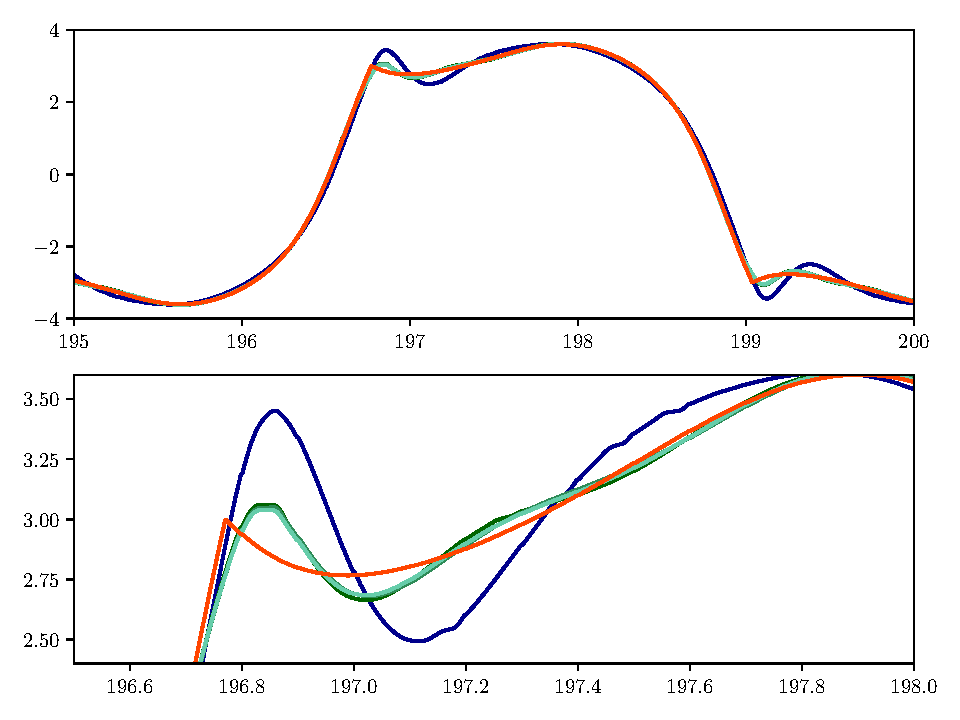
\includegraphics[width=0.8\textwidth]{Figs/Chapter8-9/preprocessing_ctrl_action.pdf}
	\caption{\textbf{Top:} Value of the real feedforward term $\uu\s\lp \ww(t) \rp$ (orange line) and of its approximations $\hat{\actfun} \lp \im(t) \rp$,
	along the system trajectory. The blue line shows the steady-state friend provied by the linear identifier,
	while the green lines report the gaussian-based identifier estimation with $N = 50$ (dark green line),
	$N = 100$ (green line), and $N = 200$ (light green line).
	\textbf{Bottom:} zoom-in to highlight the difference in the case of gaussian-based identifier with different number of samples.
	The reported quantities are plotted with respect to the time in seconds (abscissa).}
	\label{FIG:OR-PREPROCESSING-CTRL}
\end{figure}
%%%%%%%%%%
%%%%%%%%%%
\begin{figure}[!t]
	\centering
	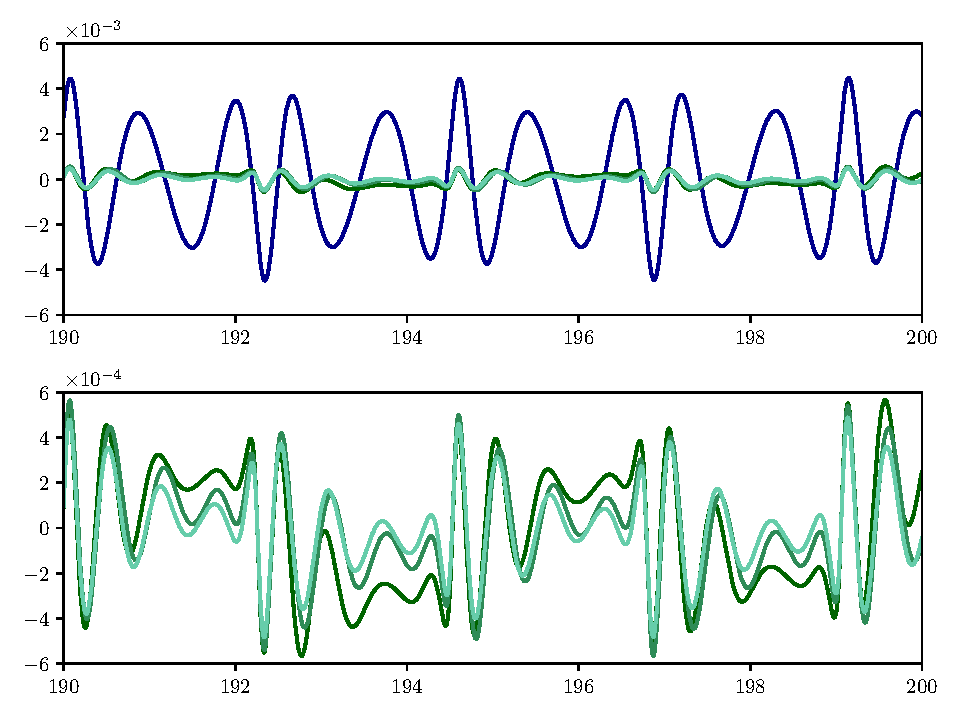
\includegraphics[width=0.8\textwidth]{Figs/Chapter8-9/preprocessing_errors.pdf}
	\caption{\textbf{Top:} steady-state evolution of the tracking error $\yy(t)$ in the two cases obtained by employing a linear identifier (blue line),
	and a gaussian-based identifier with $N = 50$ (dark green line), $N = 100$ (green line), and $N = 200$ (light green line).
	\textbf{Bottom:} zoom-in to highlight the error behavior.
	The reported quantities are plotted with respect to the time in seconds (abscissa).}
	\label{FIG:OR-PREPROCESSING-ERRORS}
\end{figure}
%%%%%%%%%%
%%%%%%%%%%
\begin{figure}[!t]
	\centering
	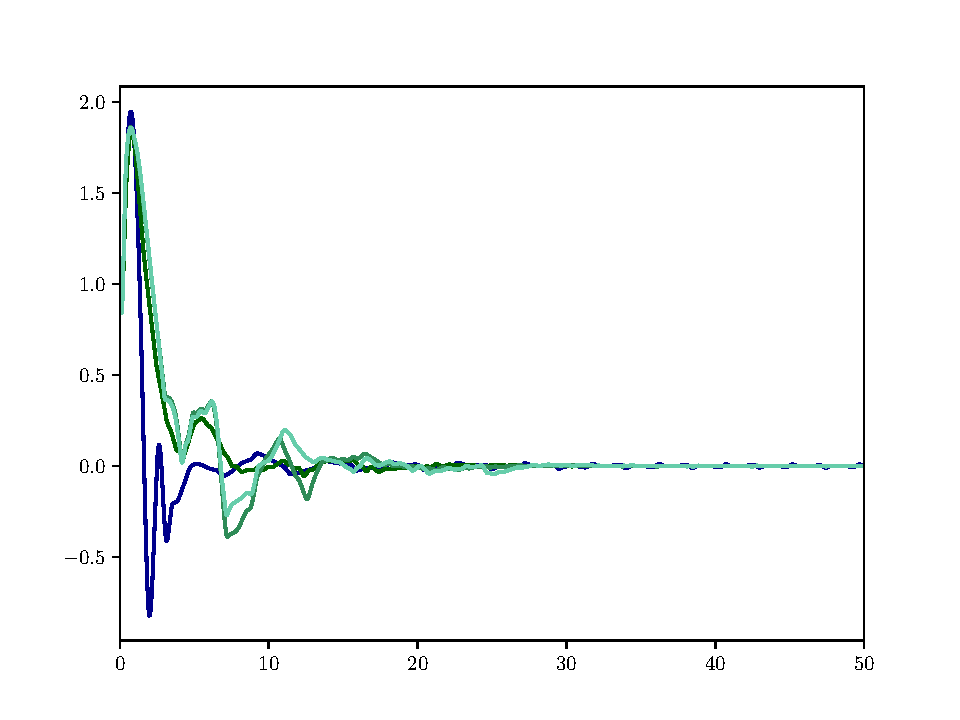
\includegraphics[width=0.8\textwidth]{Figs/Chapter8-9/preprocessing_errors_full.pdf}
	\caption{The transient evolution of the tracking error $\yy(t)$ in the two cases obtained by employing a linear identifier (blue line),
	and a gaussian-based identifier with $N = 50$ (dark green line), $N = 100$ (green line), and $N = 200$ (light green line).
	The reported quantities are plotted with respect to the time in seconds (abscissa).}
	\label{FIG:OR-PREPROCESSING-ERRORS-FULL}
\end{figure}
%%%%%%%%%%
To test the proposed regulator performances against state-of-the-art output regulation solutions, we consider the same problem
proposed by~\cite{bin2020approximate} where the output of a Van der Pol oscillator, with unknown parameter, must be synchronized with a 
triangular wave with unknown frequency.
The forced Van der Pol oscillator is described by the following equations
\begin{equation}%
   \label{EQ:PREP-VAN-DER-POL}
   \begin{split}
      & \dot{\chi}_1 = \chi_2, \\
      & \dot{\chi}_2 = - \chi_1 + a \lp 1-\chi_1^2 \rp \chi_2 + \uu,
   \end{split}
\end{equation}
with $a$ scalar unknown parameter regulating the system damping.
Furthermore, a triangular wave can be generated by an exosystem of the form
\begin{equation*}
   \begin{matrix}
      \dot{\ww}_1 = w_2, & \dot{\ww}_2 = - \varrho \ww_1,
   \end{matrix}
\end{equation*}
with output
\begin{equation*}
   \chi\s \lp \ww \rp = \frac{2 \sqrt{\ww_1^2 + \ww_2^2}}{\pi} \arcsin \lp \frac{\ww_1}{\sqrt{\ww_1^2 + \ww_2^2}} \rp,
\end{equation*}
with scalar parameter $\varrho$ the unknown oscillating frequency.
The goal is to steer the output $\chi_1$ of~\eqref{EQ:PREP-VAN-DER-POL} to the reference $\chi\s\lp\ww\rp$.
The error coordinates $\ee$ are thus defined as
\begin{equation*}
   \begin{pmatrix}
      \ee_1 \\ \ee_2
   \end{pmatrix} =
   \begin{pmatrix}
      \chi_1 - \chi\s\lp\ww\rp \\ \chi_2 - L_{\wfun\lp\ww\rp} \chi\s\lp\ww\rp
   \end{pmatrix},
\end{equation*}
and the error system reads as
\begin{equation}%
   \label{EQ:PREP-ERROR-SYSTEM}
   \begin{split}
      & \dot{\ee}_1 = \ee_2, \\
      & \dot{\ee}_2 = -\ee_1 - \chi\s - L_{\wfun\lp\ww\rp}^2 \chi\s \\
      & \hspace{1.0cm} + a \lp 1 - \lp \ee_1 + \chi\s\lp\ww\rp\rp^2 \rp \lp \ee_2 + L_{\wfun\lp\ww\rp}\chi\s\lp\ww\rp \rp.
   \end{split}
\end{equation}
The system~\eqref{EQ:PREP-ERROR-SYSTEM} is in the same form of~\eqref{EQ:PREP-FRAMEWORK} with~\assumptionref{ASSUM:REGULATOR-EQUATIONS} trivially fulfilled
since the $\zz$ dynamics is absent. Furthermore,~\assumptionref{ASSUM:CONTINUITY-ASSUMPTION} and~\assumptionref{ASSUM:STABILIZABILITY-ASSUMPTION}
hold with $\bs{\bfun} = 1$ and any $\mu \in (0,1)$. To be compliant with the results presented by~\cite{bin2020approximate} we exploit the same controller parameters
\begin{enumerate}
   \item $\kappa_s \lp \hat{\ee} \rp = K \hat{\ee}$ with $K$ such that $\sigma \lp A - BK \rp = \{-1, -2\}$, and the input $\uu$ has been saturated inside the interval $[-100, 100]$.
   \item The internal model dimension is $\dd{\im} = 2(\dd{\ww}+1) = 6$, and the matrices $F$ and $G$ has been fixed as
   \begin{equation*}
      \begin{matrix}
         F =
         \begin{pmatrix}
            -1 & 1 & 0 & 0 & 0 & 0 \\
            0 & -1 & 1 & 0 & 0 & 0 \\
            0 & 0 & -1 & 1 & 0 & 0 \\
            0 & 0 & 0 & -1 & 1 & 0 \\
            0 & 0 & 0 & 0 & -1 & 1 \\
            0 & 0 & 0 & 0 & 0 & -1
         \end{pmatrix}, &
         G = 
         \begin{pmatrix}
            0 \\ 0 \\ 0 \\ 0 \\ 0 \\ 1
         \end{pmatrix}.
      \end{matrix}
   \end{equation*}
   \item The control parameters has been chosen as $l = 20$, $h_1 = 6$, $h_2 = 11$, $h_3 = 6$, and $\underline{\TT} = \overline{\TT} = 0.1$.
\end{enumerate}
The simulations reported in Figures~\ref{FIG:OR-PREPROCESSING-ERRORS},~\ref{FIG:OR-PREPROCESSING-ERRORS-FULL}, and~\ref{FIG:OR-PREPROCESSING-CTRL} show the proposed regulator applied
with $a = \varrho = 2$ in three cases with $N = 50$, $N = 100$, and $N = 200$. The obtained results are then compared with the regulator proposed
by~\cite{bin2020approximate} where the identifier is chosen as a least-squares identifier working on the model set
$\MM = \left\{ \imfunsingle \lp \param, \im \rp: \R^{\dd{\im}} \mapsto \R^{\dd{\yy}} | \imfunsingle \lp \param, \im \rp = \param\T\im, \param \in \paramset \subset \R^{\dd{\im}} \right\}$.
In all simulations the GP parameters has been kept fixed at $\nn = 0.01$ and $\pvar_{\text{thr}} = \np = 1$, while the kernel hyperparameters
$\boldsymbol{\lambda} = (\lambda_{\im_{1}}, \dots, \lambda_{\im_{\dd{\im}}})$ has been estimated via log-likelihood minimization \cite{rasmussen2003gaussian}
yielding to the values of $\boldsymbol{\lambda} = \lp 7.7, 34.3, 19.9, 0.4, 133.6, 1.2 \rp$. As emerges from~\figref{FIG:OR-PREPROCESSING-ERRORS}, the proposed approach
reduces the maximum error of more than $100$ times compared to the case with least-square identifier.

%----------------------------------------------------------------------------------------
\section{Contributions}
We presented two learning-based techniques to design internal model-based regulators for a large class of nonlinear systems.
The proposed techniques fit in the general frameworks recently proposed in~\cite{bin2019class} and~\cite{bin2020approximate}, and
shows how the identification of the optimal steady state control input can be performed by using Gaussian process
models. The flexibility of the proposed approaches make the regulator able to deal with highly uncertain shapes of the optimal steady-state control input
useful to make zero the output error. Thanks to the fact that only coarse and qualitative knowledge about the friend is required, the proposed designs
may be employed as solution to many of the output regulation problems addressed in literature. 
The previous analysis also derives probabilistic bounds on the attained performances and presents numerical simulations showing
how the proposed methods outperforms state-of-the-art approaches when the regulated plant or the exogenous disturbances are subject to unmodeled perturbations.
Future research directions will be aimed at exploring deeper the Gaussian process flexibility by focusing on
the injection of possibly a priori knowledge of the friend structure, and at investigating how the proposed performance
bound changes. We also aim to investigate if Gaussian process-based internal models may deal with non minimum-phase systems.

%------------------------------------------------